\documentclass{article}


\usepackage{arxiv}

\usepackage[utf8]{inputenc} % allow utf-8 input
\usepackage[T1]{fontenc}    % use 8-bit T1 fonts
\usepackage{hyperref}       % hyperlinks
\usepackage{url}            % simple URL typesetting
\usepackage{booktabs}       % professional-quality tables
\usepackage{amsfonts}       % blackboard math symbols
\usepackage{nicefrac}       % compact symbols for 1/2, etc.
\usepackage{microtype}      % microtypography
\usepackage{lipsum}
\usepackage{graphicx}
\graphicspath{ {./images/} }

\usepackage{lmodern}%
\usepackage{textcomp}%
\usepackage{lastpage}%
% \usepackage[margin=0.5in]{geometry}%
\usepackage{float}%
\usepackage{xcolor}
\usepackage[export]{adjustbox}
\usepackage[numbers]{natbib}
\usepackage{listings}
\usepackage{minted}
\usemintedstyle{vs}
\usepackage{subfig}
\usepackage{multirow}


\title{Accelerated Atomistic Modelling of Aluminum Precipitates: A Case Study with Al-Cu}

\author{
 Daniel Marchand \\
  Institute of Materials Science \\
  École Polytechnique Fédérale de Lausanne \\
  CH-1015, Vaud, Switzerland \\
  \texttt{daniel.marchand@epfl.ch} \\
  %% examples of more authors
   \And
 Albert Glensk \\
  Institute of Mechanical Engineering \\
  École Polytechnique Fédérale de Lausanne \\
  CH-1015, Vaud, Switzerland \\
  \texttt{albert.glensk@epfl.ch} \\
  \And
 William Curtin \\
  Institute of Mechanical Engineering \\
  École Polytechnique Fédérale de Lausanne \\
  CH-1015, Vaud, Switzerland \\
  \texttt{william.curtin@epfl.ch} \\
  %% \AND
  %% Coauthor \\
  %% Affiliation \\
  %% Address \\
  %% \texttt{email} \\
  %% \And
  %% Coauthor \\
  %% Affiliation \\
  %% Address \\
  %% \texttt{email} \\
  %% \And
  %% Coauthor \\
  %% Affiliation \\
  %% Address \\
  %% \texttt{email} \\
}

\begin{document}
\maketitle
\begin{abstract}
Precipitates are fundamental to the strengthening of aluminum alloys, and understanding them is paramount for optimized processing.
Precipitates are highly complex, and their formation sequence, kinetics, and the resulting influence on mechanical properties must be studied at the atomic scale, particularly during early-stage nucleation and growth.
Atomistic modeling via Density Functional Theory (DFT) is well-established and has been successful for a wide variety of precipitates; however, it is extremely computationally expensive and typically limited to modeling relatively simple bulk properties. On the contrary, interatomic potentials are computationally affordable, yet tend to lack accuracy. A promising new method for modeling precipitates is through the use of interatomic Neural Network Potentials (NNPs), that have near-DFT accuracy without the massive cost. 
Here, we present a demonstration of NNPs for Al-Cu based-alloys, their >$\theta$ precipitation sequence being one of the oldest and most investigated in the field, providing a model system for comparison.
We demonstrate the high fidelity of the Al-Cu NNPs for predictions of intermetallic compound energetics, elasticity, dilute solid-solution binding, interfaces, generalized stacking fault energy surfaces, and anti-site defect energies.
We further show that our NNP can correctly the entropically-induced shift between $\theta'$ and $\theta$, 
\textcolor{red}{I AM TENTATIVELY ADDING A KMC SECTION SINCE ABHINAV'S RESULTS SEEM PROMISING} while with Kinetic Monte Carlo we show our NNP can model early-stage GP \textcolor{red}{AND GP2?} zone formation.
This work points to a new and powerful approach for advancing the predictive understanding of Al alloys. 
\end{abstract}


% keywords can be removed
%\keywords{First keyword \and Second keyword \and More}


\section{Introduction}
Aluminum is one of the critical materials in the modern world.
Pure Aluminum is almost useless because of its low yield point\cite{Nie2014PhysicalAlloys}; defects are what give Aluminum its utility, its strength.
Precipitates are, arguably, the most essential, and most complex defects for understanding Aluminum's mechanical properties.
Heat is almost always needed to obtain the optimal type and size of precipitates, so much heat, that aluminum production is one of the largest energy-consumers of the planet\cite{Raabe2019StrategiesMetals}.
It is not trivial to predict the amount of heat needed, or even the concentration of elements to add, as the mechanical properties are the unique function of dozens of alloying elements and innumerable processing conditions.

Good atomic models are essential in the study of aluminum precipitates, firstly, because the initial formation of precipitates involves small clusters of atoms, too small to be viewed with ease in experiments.
Secondly, because the interactions between dislocations and small precipitates are discrete, and does not readily lend itself to continuum modeling.
The challenge is to find atomic models that are both accurate and fast.
Density Functional Theory (DFT) is very accurate, but incredibly slow modeling more than a few hundred atoms in DFT is exceptionally challenging\cite{Martin2004}.
Atomic potentials are fast, but often inaccurate, it is challenging to have atomic potentials model all of the properties relevant to precipitate formation, growth, and influence on mechanical properties[REF].

In this work, we focus on Al-Cu as a case study for atomic modeling.
It has been well-studied for a long time\cite{Preston1938StructureAlloys}, thus making it nicely comparable for benchmarks.
Furthermore, it exhibits several properties that are challenging to model, notably the entropically-driven $\theta'$→ $\theta$ transformation \cite{Wolverton2001b}.

Apostol and Mishin created an Angular Dependent Potential (ADP) for Al-Cu systems.
In their work, they focused on modeling: formation energies, lattice constants, elastic constants, surface energies, and generalized stacking fault energies\cite{Apostol2011}.
The potential became very popular and was used in numerous studies of mechanical behavior of precipitates,
in studying solute and precipitate strengthening\cite{Singh2013AnAlloy}\cite{Esteban-Manzanares2019}\cite{Wu2020AtomisticAlloys}.
Work by Kobayashi et al. \cite{Kobayashi2017} studied Al-Mg-Si with Neural Network Potentials (NNPs), and they had found excellent results in modeling precipitate-relevant properties beyond what was possible with other potentials for that system.

Our goal in this work was to attempt to construct an NNP that would improve state of the art in precipitate modeling, where we use ADP a comparison.
We carefully, systematically examined all the atomic-level properties that would be relevant to precipitate modeling: solute/vacancy interactions, formation energies, elastic constants, interface energies, generalized stacking fault energies and the as-mentioned entropic stability of $\theta'$ over $\theta$ phase.

\section{Methodology}
NOTE: I probably don't need the actual subsection headers. 
\subsection{DFT Training Set Generation}
\subsection{NNP selection and Evaluation of Errors}
In this work, we trained several NNPs (N=40) to estimate expected errors. We selected the NNP with the lowest error for $C_{44}$ in aluminum to be the single representative example because of the importance and relative difficulty, as will be discussed later, of modeling $C_{44}$ correctly. All error bars center on the average of all trained NNPs and extends their standard deviation outwards. Thus, the representative NNP, i.e., the NNP with the closest $C_{44}$ to DFT, is not always close to the error bar center, nor does it always lie within the error bars. 
\subsection{Atomic Structures}
The Open Quantum Materials Database \cite{Kirklin2015} was the primary source of structures used when training and
testing the NNP across a broad range of Al-Cu compounds. $\theta$ and $\theta''$ were not in the OQMD, and we
included them as well manually for a total of 62 structures. Each of these structures was then fully relaxed, 
both in cell dimensions and atomic positions. Because we wished to avoid testing duplicates, only structures that retained the same symmetry group before and after relaxation were explicitly compared against the ADP and NNP
potentials (N=47). The elastic tensor was computed similarly to \cite{DeJong2015}, where a finite set of strains were
applied and fitted to the associated stresses. The pymatgen package\cite{Ong2013} determined the minimal number of
deformations required for each structure based on its symmetry, and only these were used. 
Unless stated otherwise, we computed formation energies using FCC Al and FCC Cu as the corresponding ground states. 

\textcolor{red}{We made heavy use of the atomic simulation environment for the generation of structures, and for evaluating energies using ADP and NNP \cite{HjorthLarsen2017}}

\section{Results and Discussion}
\subsection{NNP Evaluation}
\textcolor{red}{TODO: here place the a plot of DFT vs NNP structure energies.
In our test, the validation error was much much higher than the training error.
You will need to explain this due to outliers and discuss their relevancy. }

Figure \ref{fig:matparam_purestats} shows the performance of NNP and ADP against DFT on fundamental properties: lattice and elastic constants, surface and stacking fault energies, for pure Al and Cu.
For most of these properties, NNP shows little or no advantage relative to ADP, the sole exception being stable stacking fault energies in aluminum.
Troublingly, the $C_{44}$ values of aluminum are substantially and statistically different from those of DFT.
This error is not entirely unusual for NNPs, and prior work has found errors of a similar magnitude\cite{Zuo2020APotentials}.
On theoretical grounds, elastic constants are a function of the second derivative of energy, and one should expect to be correspondingly much harder to accurately model when training primarily on energies.
Because we have used a very dense kpoint mesh, and we have systematically used the same settings, we do not expect this error in $C_{44}$ to be due to issues in the underlying training set, as was found to be a critical factor for a machine-learning we potential based on iron \cite{Dragoni2018AchievingIron}.  
In any case, we find that our potential is highly performant when one is considering a broad range of structures, or when one is evaluating energetics of complex geometries. 

\begin{figure}[H]%
\centering%
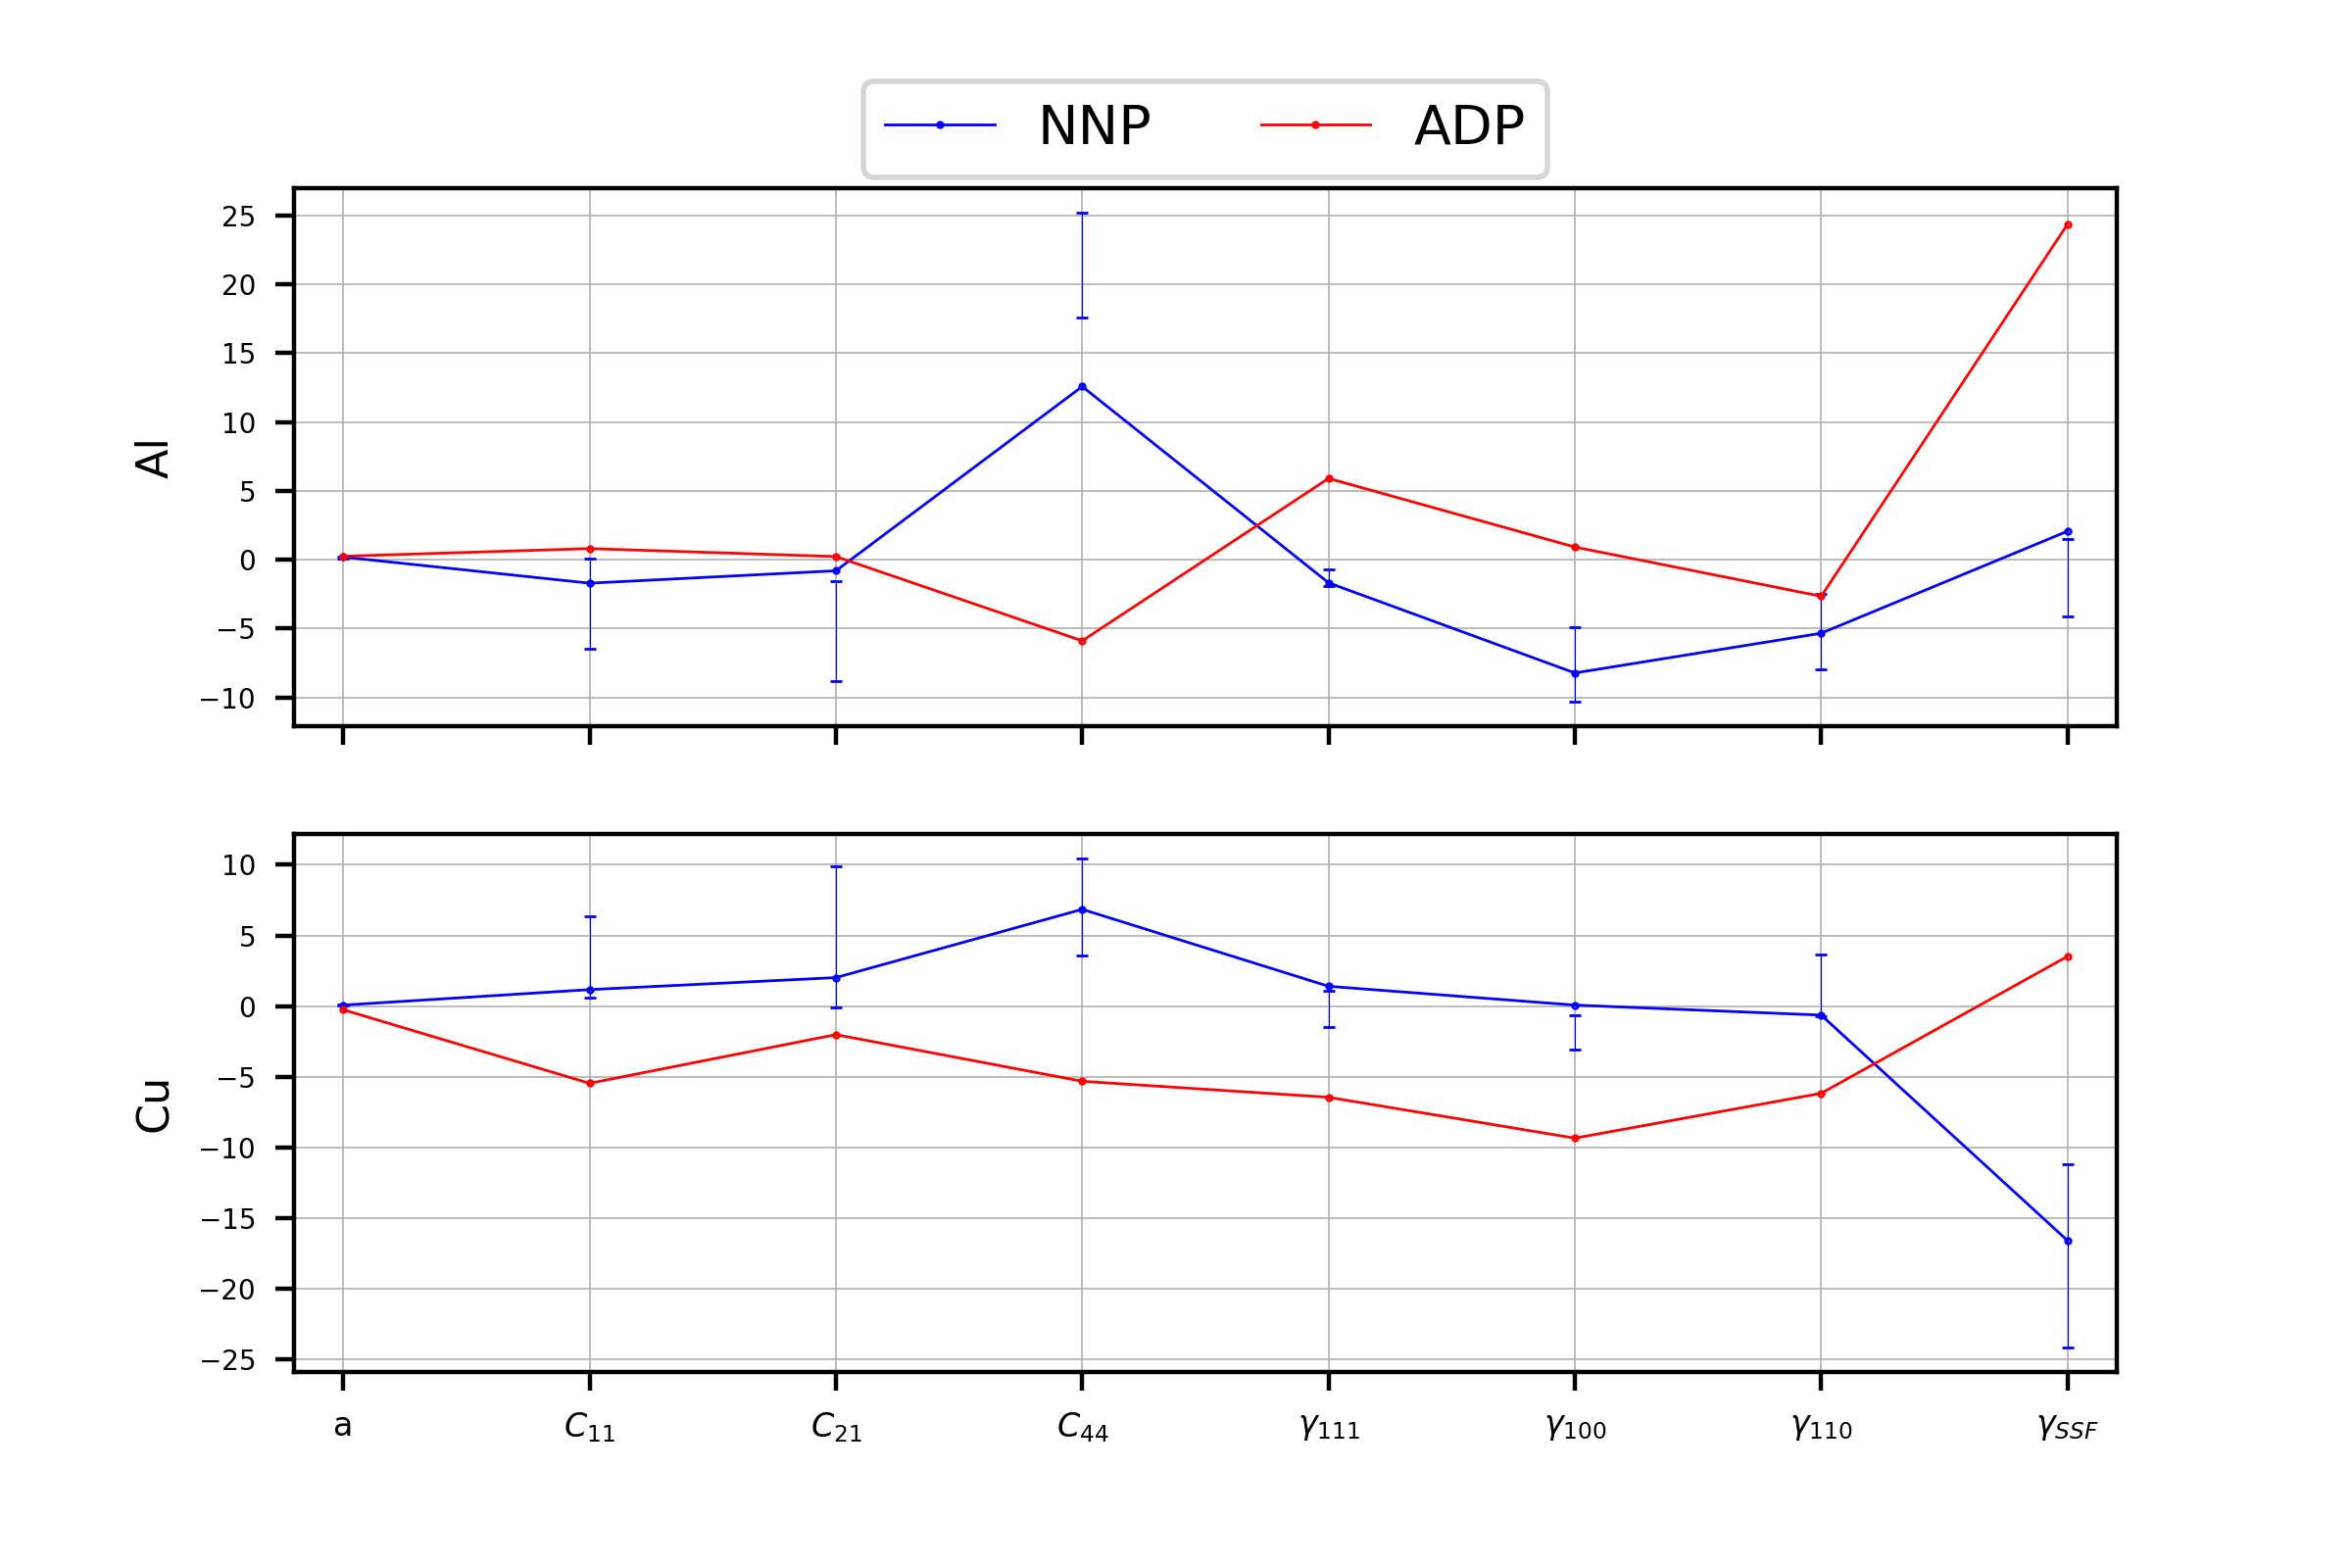
\includegraphics[width=1.2\textwidth,center]{./figures/matparam_purestats.png}%
\caption{Deviation of NNP and ADP from DFT (\%) for fundamental properties for Al and Cu. 
Relevant structures are included in the training set. }%
\label{fig:matparam_purestats}
\end{figure}
The NNP outperforms ADP for formation energy, atomic volume, and elastic constants for most OQMD structures, as can be seen in Figure \ref{fig:matparam_stats1}.
Formation energy is particularly well-handled by the NNP, with most errors well within a few meV/atom, while ADP often highly overestimates or underestimates the formation energy;
in a few cases, ADP reverses the sign, i.e., predicting stable compounds as unstable and vice versa.
However, for structures with high formation energy, both the NNP and ADP tend to struggle, often they do not end up relaxing to the same structure as DFT, or they have substantial errors.
ADP regularly underestimates the atomic volume, even for critical structures: $\theta$ and $\theta'$ errors can be substantial, see \textcolor{red}{supplamentary table}.
For elastic constants, we see that neither ADP nor NNP performs ideally.
ADP does a reasonable job of capturing the precipitate structures and outperforms NNP on pure aluminum.
However, we see that ADP often makes quite substantial errors in the elastic constants for intermediate compounds, while this is less the case for NNP. Interestingly it seems that the B2 structure poses a challenge to both ADP and most NNP.
ADP predicts B2 to be extremely stable, while it has the highest error for any stable compound for NNP. 


\begin{figure}[H]%
\centering%
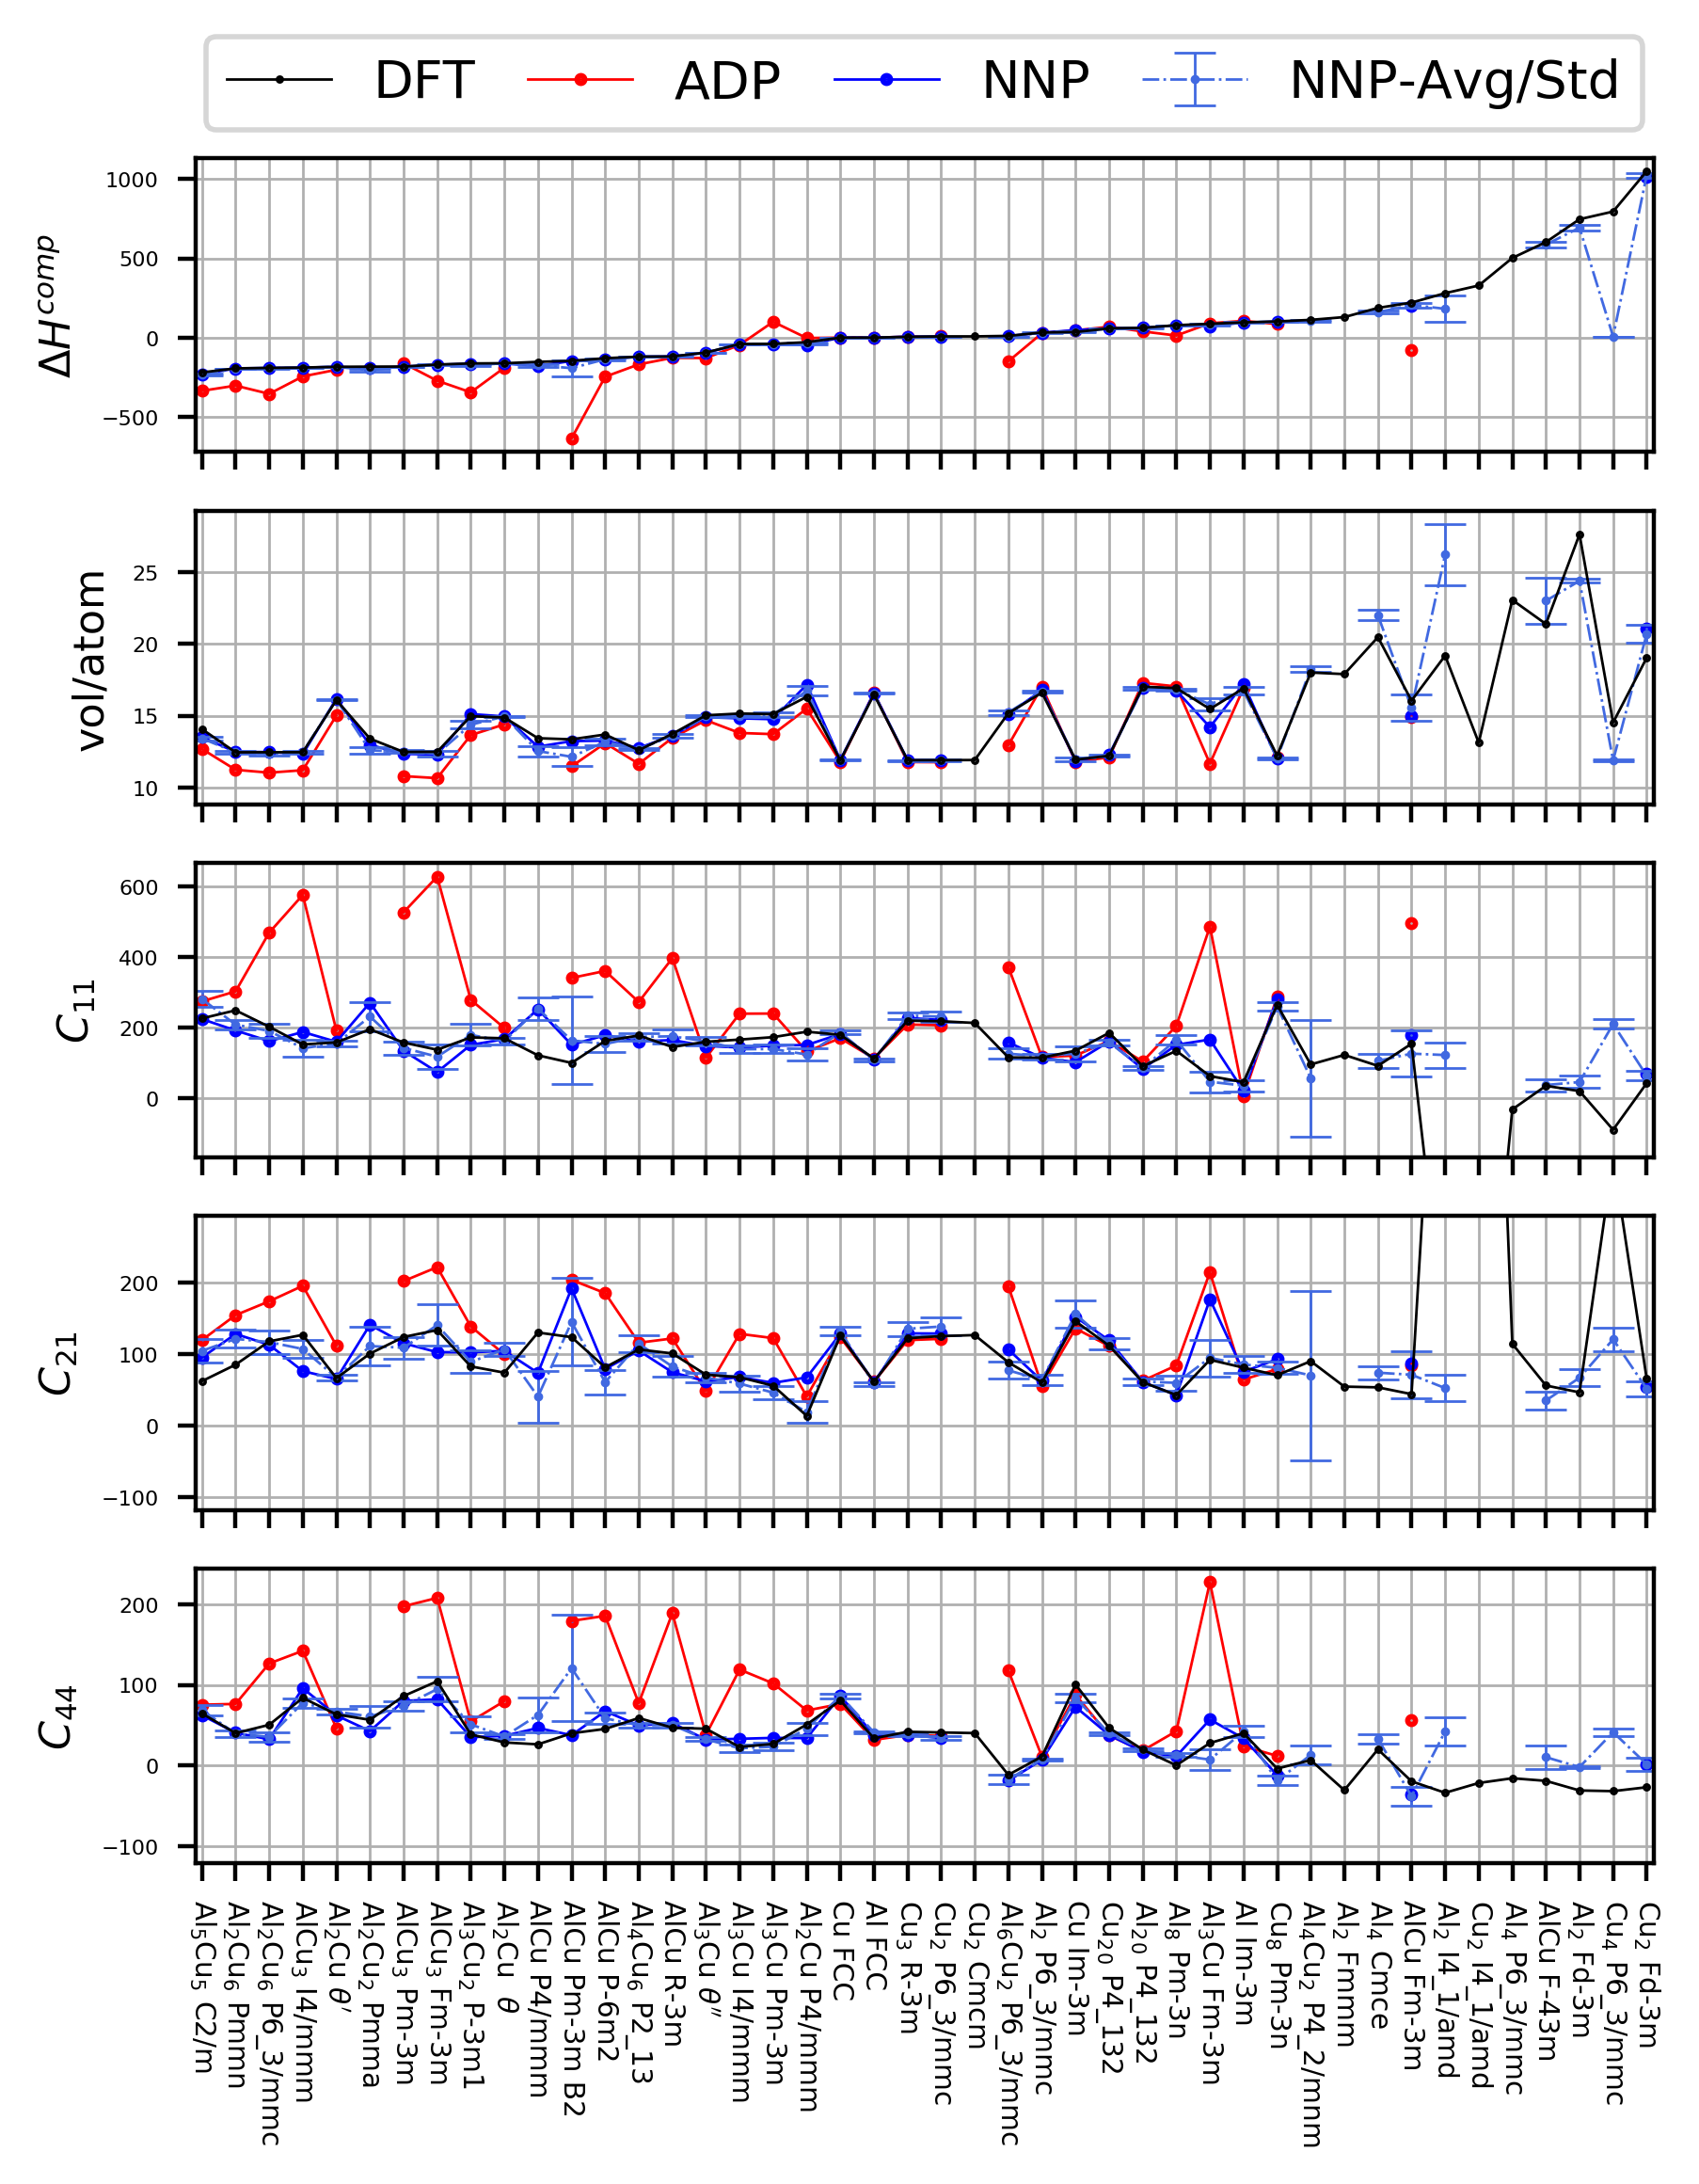
\includegraphics[width=1.2\textwidth,center]{figures/matparam_stats1.png}%
\caption{Comparison of: formation energy (meV), atomic volume (Ang$^3$), elastic constants C$_{11}$, C$_{21}$ and C$_{44}$ (GPa) across NNP, ADP and DFT for all structures in the OQMD. 
Relevant structures are included in the training set. }
\label{fig:matparam_stats1}
\end{figure}

The binding energies for Cu, Al, and Vacancy in Al or Cu matrix was computed with following:
\begin{equation}
E_{bind} = E^{2sol}_{N-2,X,Y}-E^{1sol}_{N-1,X}-E^{1sol}_{N-1,Y}+E^{pure}_N
\end{equation}
The results for Al matrix are displayed in Figure \ref{fig:solsol_in_al} while those for Cu matrix are contained in the \textcolor{red}{Figure S \ref{fig:solsol_in_cu}}.
For the solute binding, we see that the NNP, while not always ideal, more closely matches DFT.
Particularly for dilute Cu-Cu binding, ADP falsely predicts massive overbinding for near neighbors and massive repulsion for further neighbors, while NNP maintains quantitative accuracy.
Errors for NNP are typically in the 20-30 meV range, and values requiring greater precision than this would not be appropriate for NNP.


\begin{figure}[H]%
\centering%
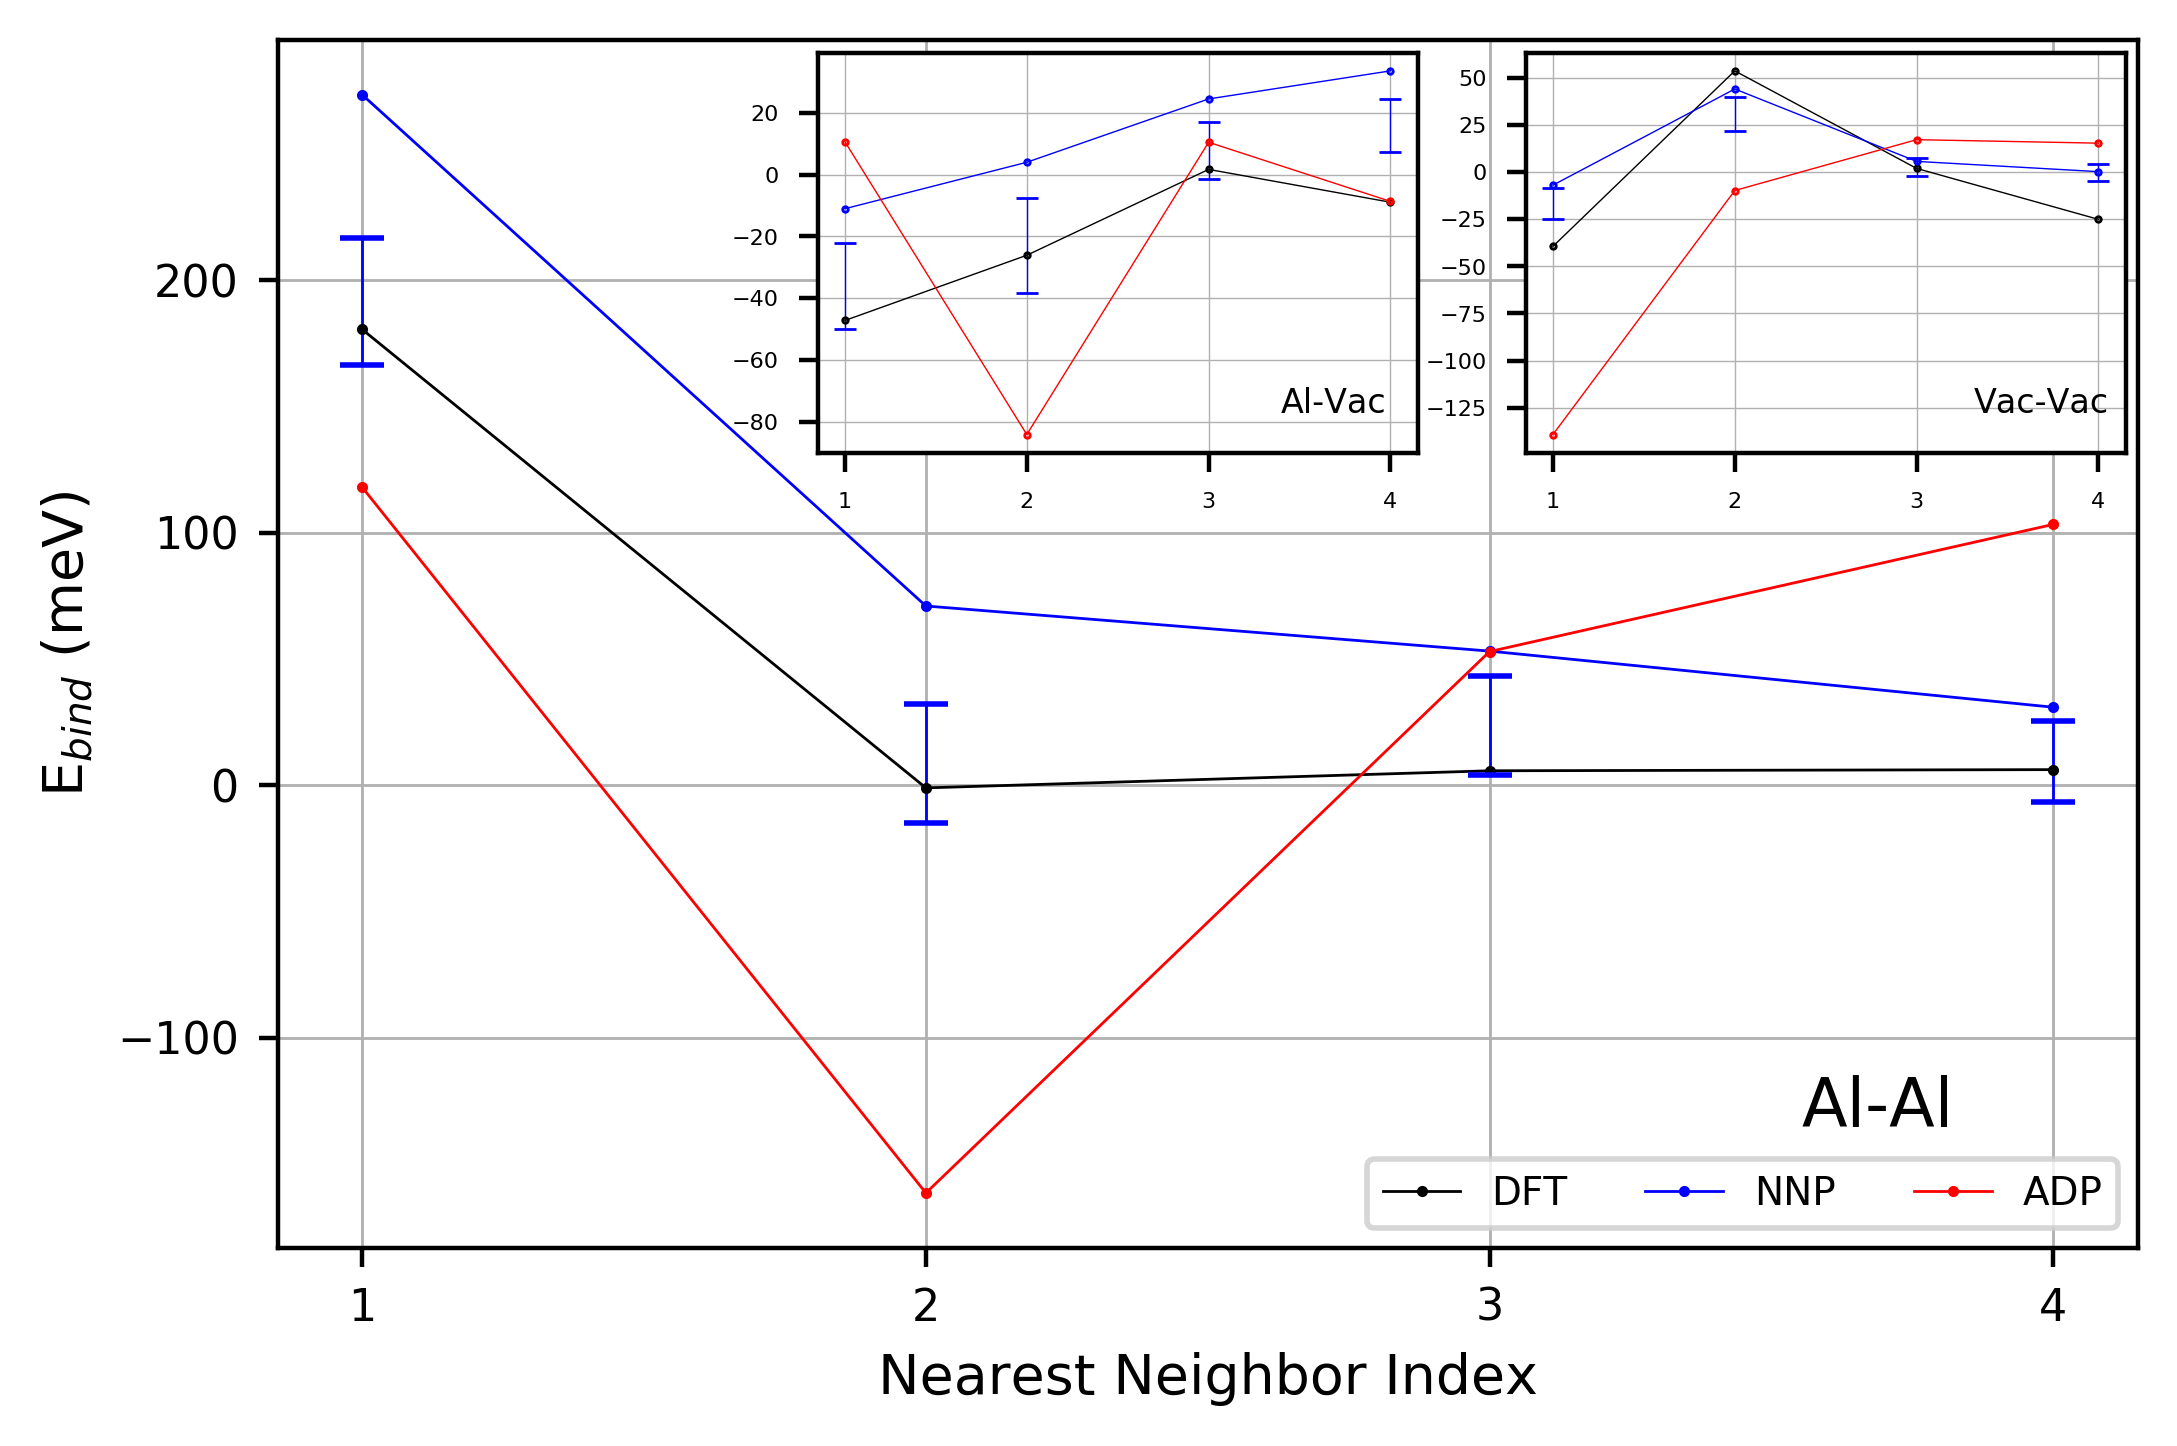
\includegraphics[width=1.2\textwidth,center]{./figures/solsol_in_al.png}%
\caption{Neighbor index vs binding energy $E_{bind}$ for Cu-Cu, Cu-Vac and Vac-Vac in Al matrix. 
Relevant structures are included in the training set.}%
\label{fig:solsol_in_al}
\end{figure}

\textcolor{red}{Not yet sure whether geometry has a separate section or not}.
In this work, the coherent and semi-coherent versions of the $\theta''$ and $\theta'$ interfaces were studied while $\theta$ was omitted since it only forms incoherent interfaces \cite{Nie2014PhysicalAlloys}.
We constructed these interfaces by taking their OQMD entries and stacking them on the Al matrix using the ASE \mintinline{python}{ase.build.stack} command.
During relaxation, atoms are free to move, but the cell is held fixed. 
Reference images for these interfaces are included in \textcolor{red}{Figure XX} in the supplementary.

We computed the interface energy in the same manner as in \cite{Vaithyanathan2004MultiscaleAlloys}, and we only briefly summarize the method here.
The formation energy for an interface with N atoms of which X are of the matrix and Y are of the precipitate,
$H^{int}f_{X,Y} = E^{int}_{X,Y}-XE^{Matrix}_{bulk}-YE^{Precip}_{bulk}$,
is related to the number of atoms in the following equation. 
\begin{equation}
H^{int}f = \delta E_{strain} + \frac{2A\gamma^{int}}{N}
\end{equation}
Where $H^{int}f$ is the interface formation energy, $\delta E_{strain}$ is the strain energy, $A$ the surface area,
$\gamma^{int}$ the interface energy, and N the total number of atoms in interface.
The interface energy $\gamma^{int}$ is then the slope of $\frac{1}{N}$ against $H^{int}f$, divided by $2A$.
We calculated the slope using three different sizes of the $\theta'$ structures and four different sizes of $\theta''$ structures, starting with a minimum of one precipitate layer and two Al layers and incriminating onward in size. 

Figure \ref{fig:interface_energies} plots the results of the interface energy calculations.
ADP correctly predicts the general trends but makes several serious errors.
The coherent $\theta'$ interface has much too high an energy, while all the $\theta''$ interface is predicted to have negative energy.
The $\theta''$ interface is particularly challenging because it has such low interface energy; therefore, it is easy for the potential to predict this to be negative rather than positive.
However, our representative NNP has high quantitative accuracy on all these interfaces.

\begin{figure}[H]%
\centering%
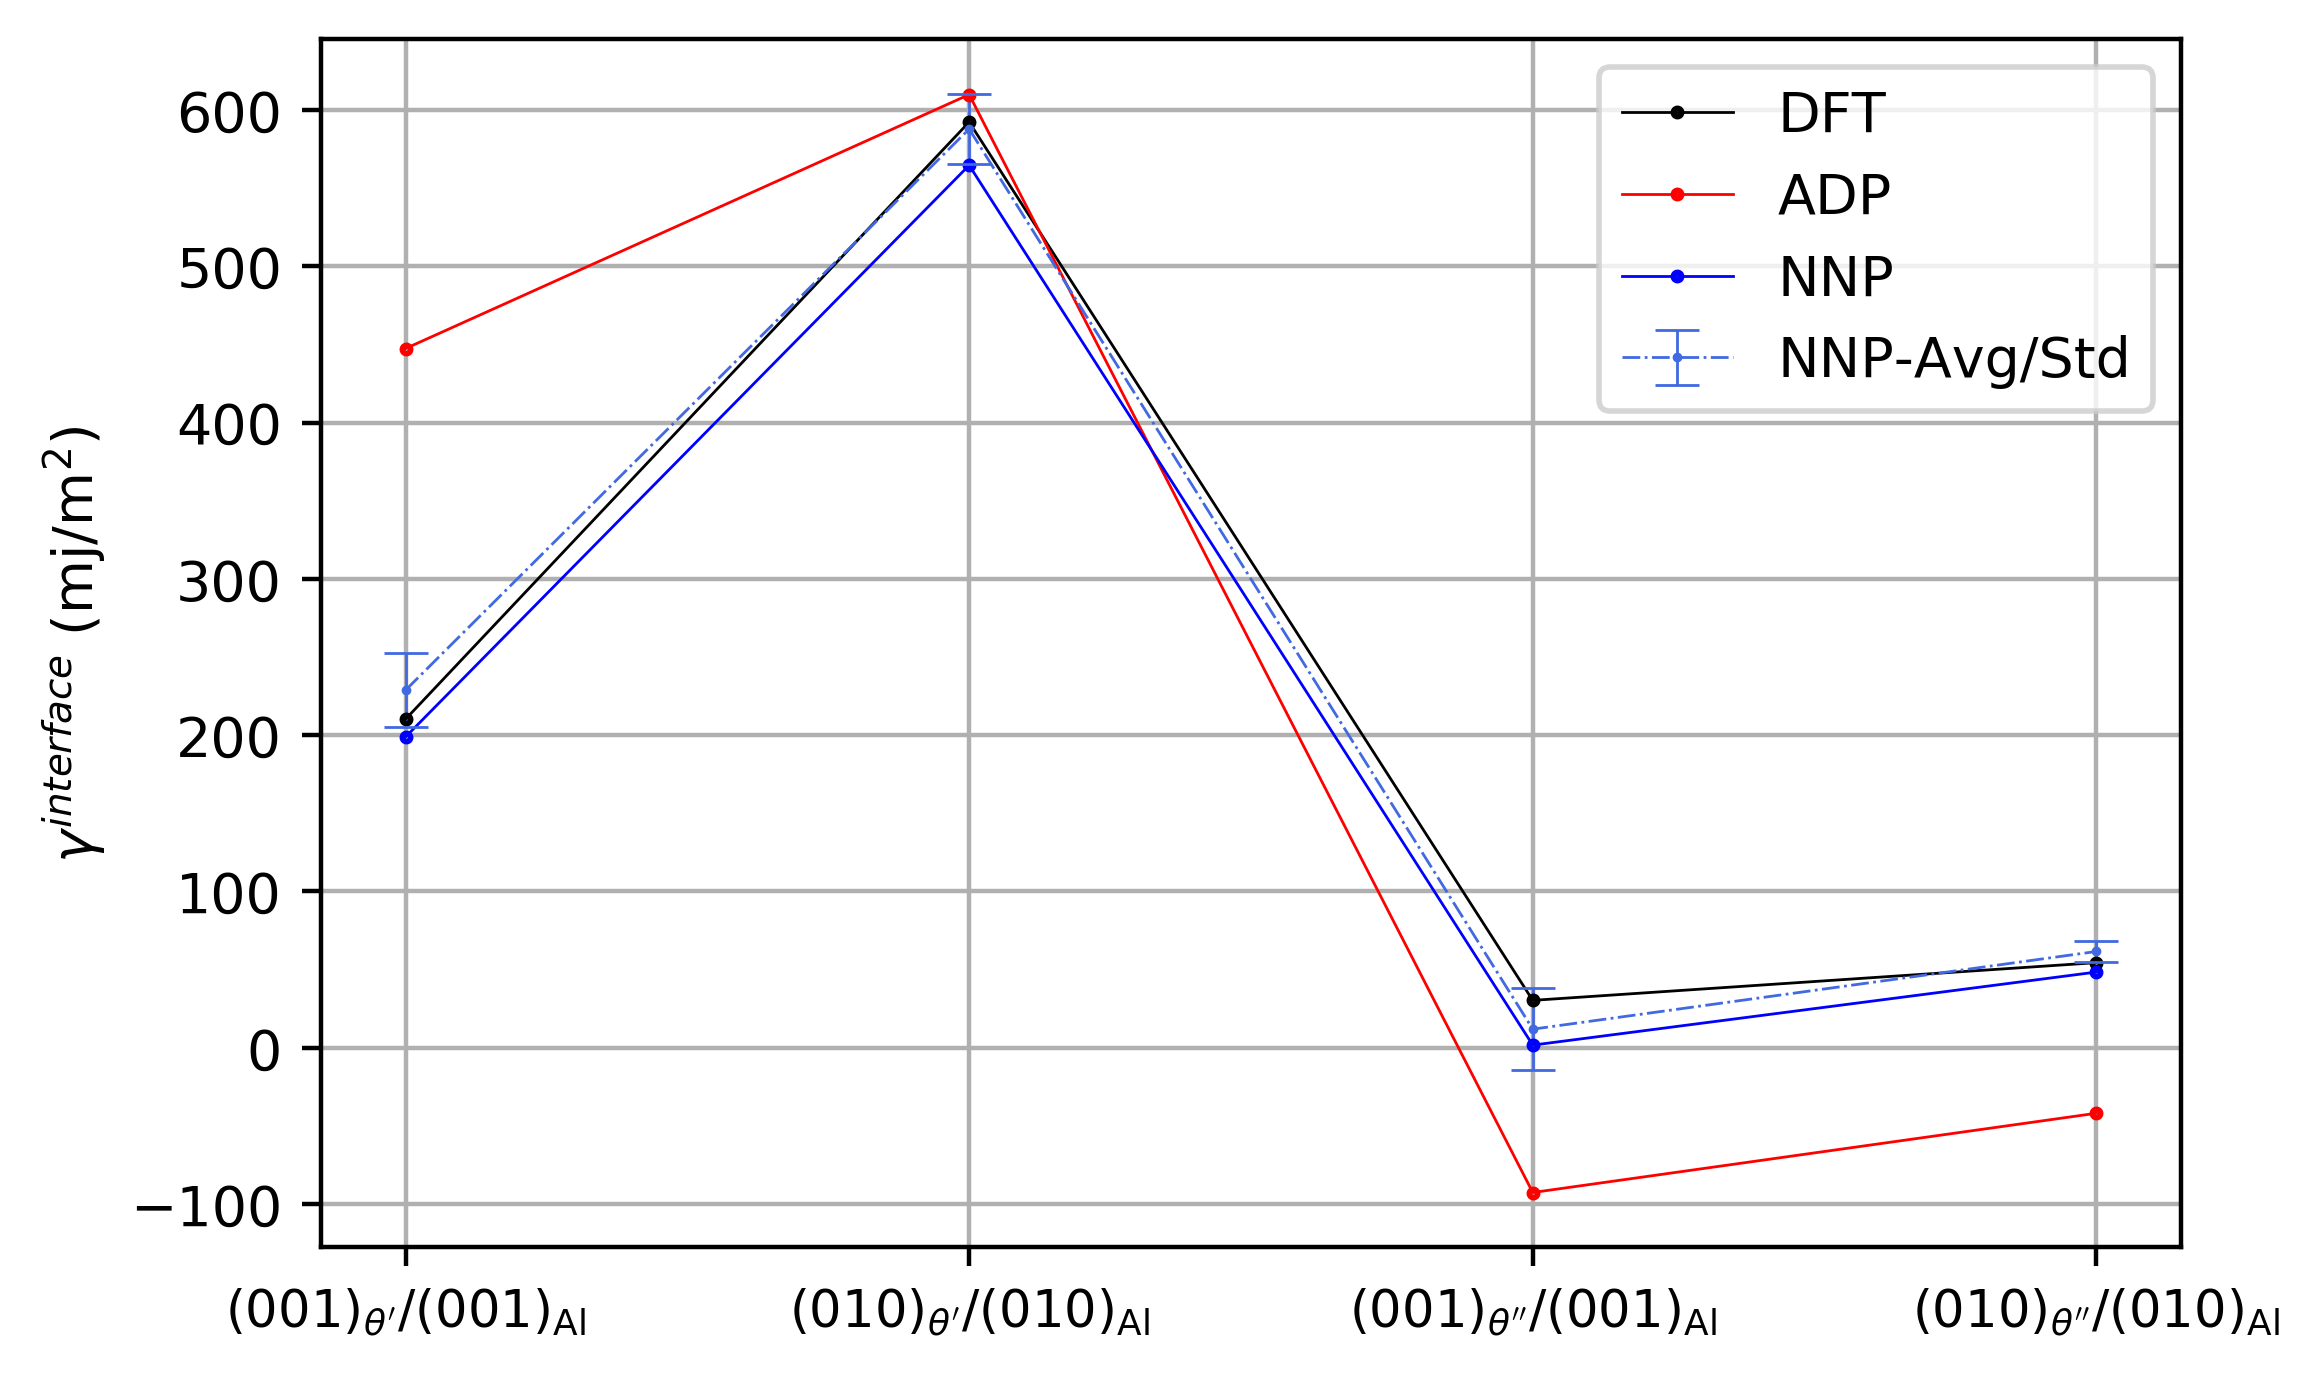
\includegraphics[width=1.2\textwidth,center]{./figures/interface_energies.png}%
\caption{Interface structure vs interface energy for precipitate structures. 
These are the $\theta'$ coherent, $\theta'$ semi-coherent, $\theta''$ coherent and $\theta''$ semi-coherent
interfaces in order. Relevant structures are included in the training set.}%
\label{fig:interface_energies}
\end{figure}

\textcolor{red}{GSF SECTION GOES HERE}
\begin{figure}[H]%
\centering%
\subfloat{{
 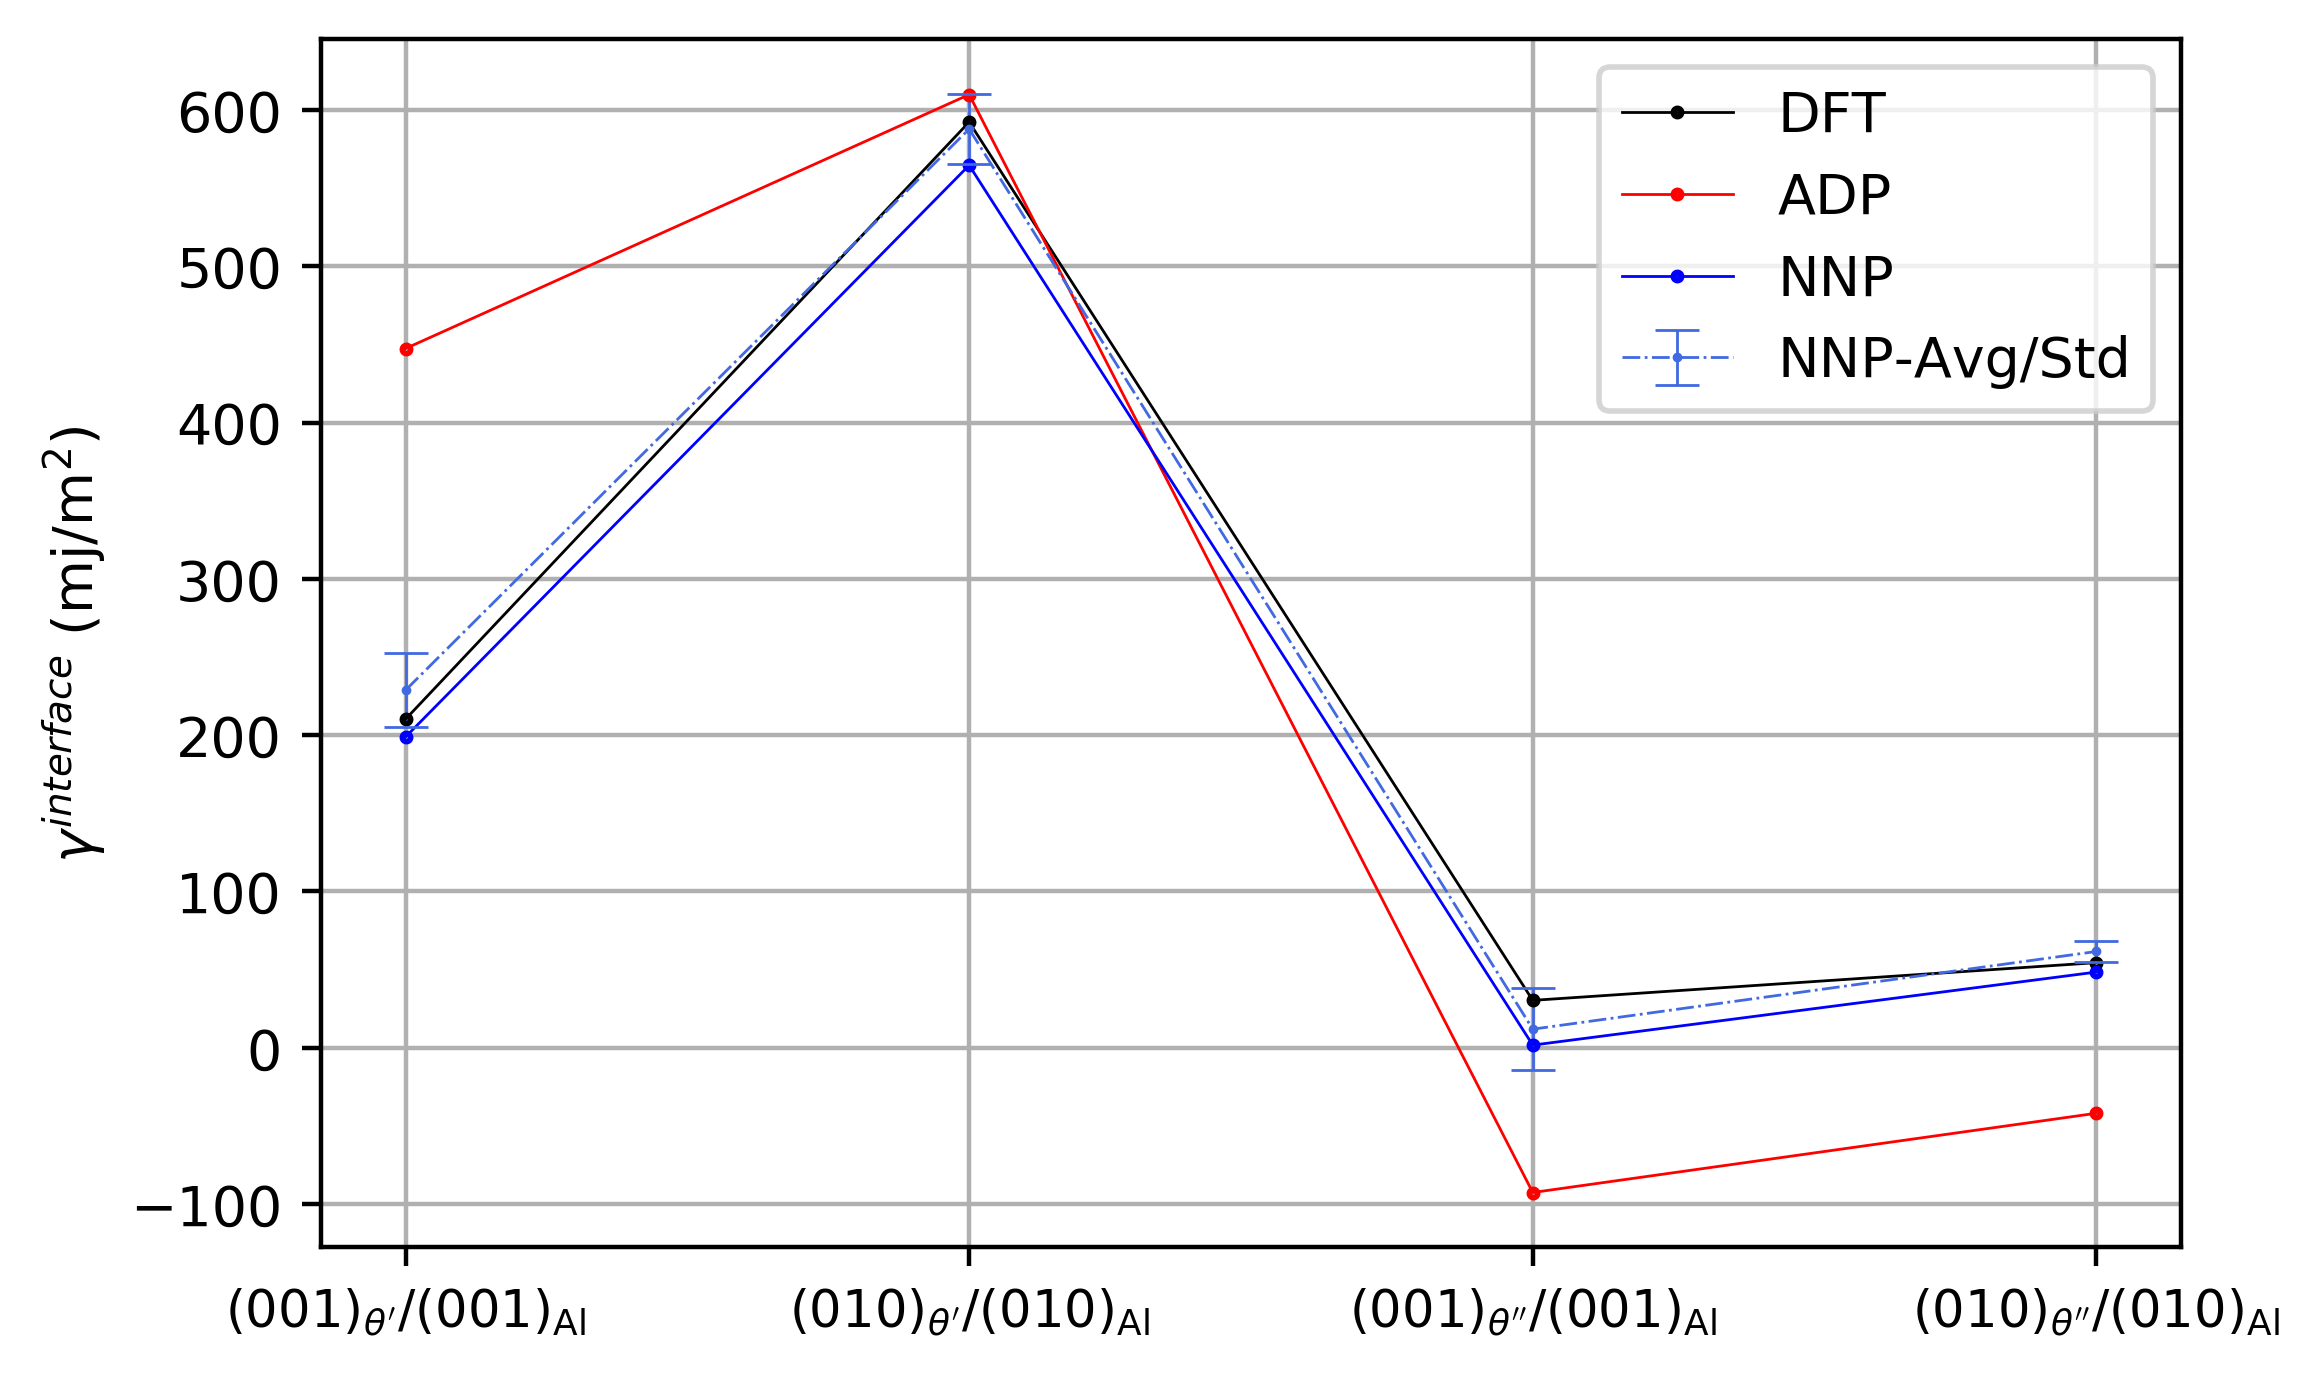
\includegraphics[scale=0.4]{./figures/interface_energies.png}
 }}%
\subfloat{{
 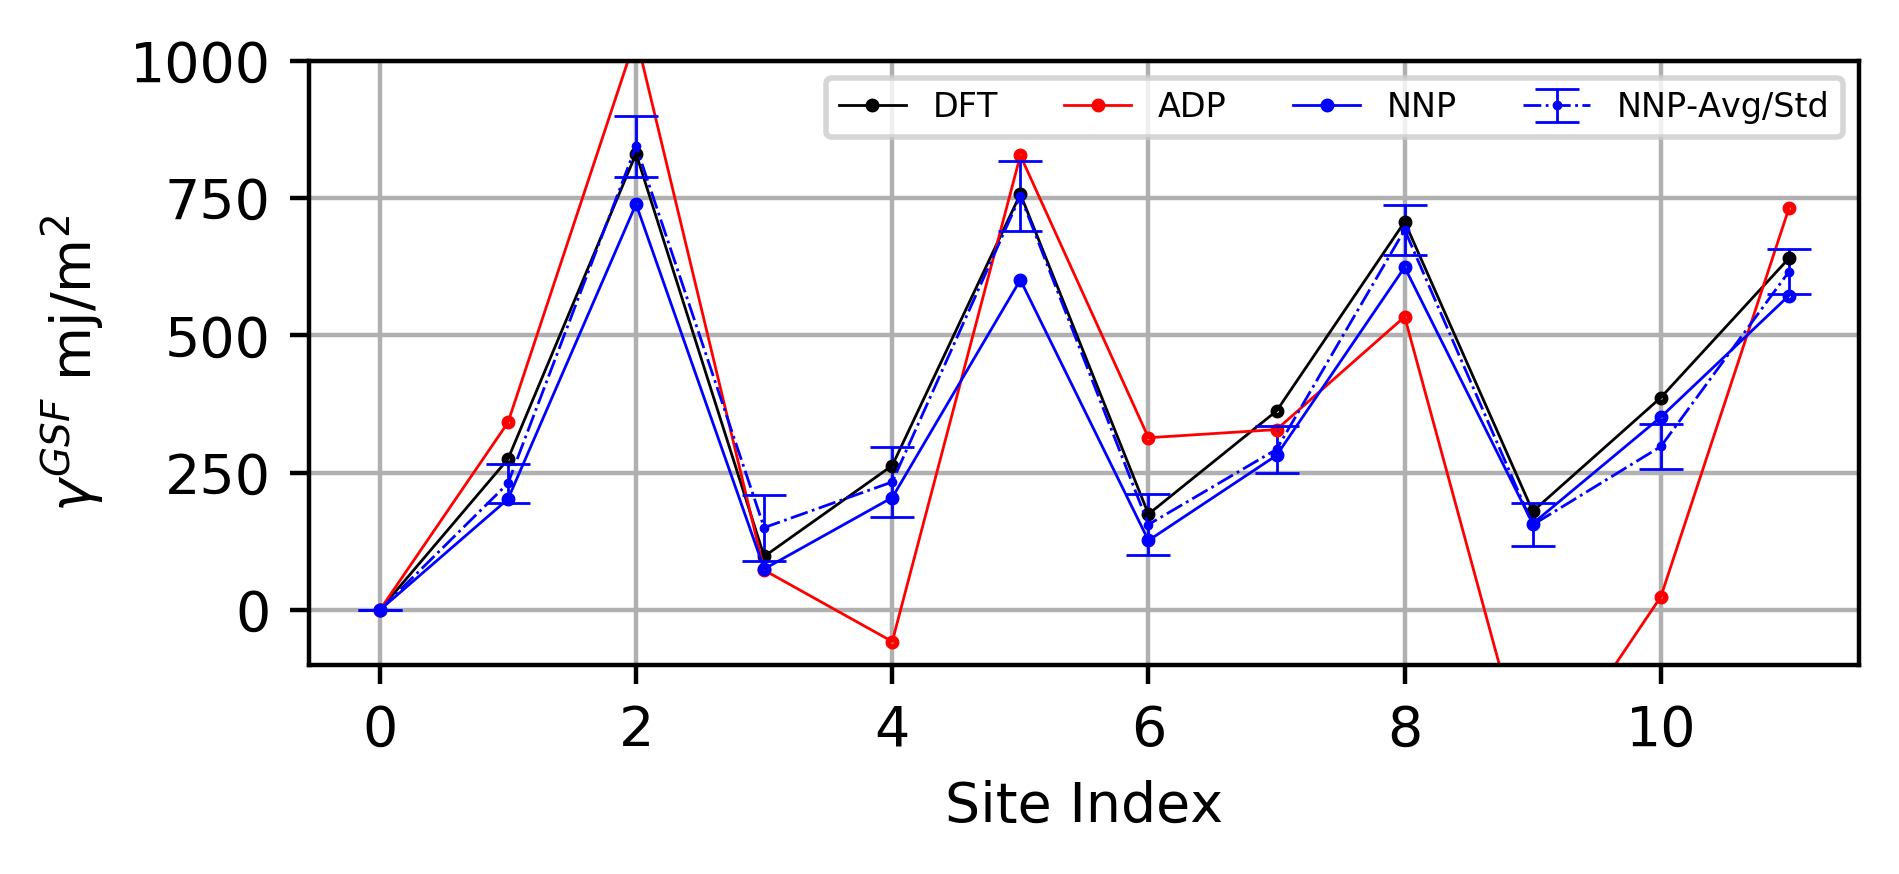
\includegraphics[scale=0.8]{figures/NOTINOQMD_00002-GSF_111.png}
 }}%
\\
\subfloat{{
 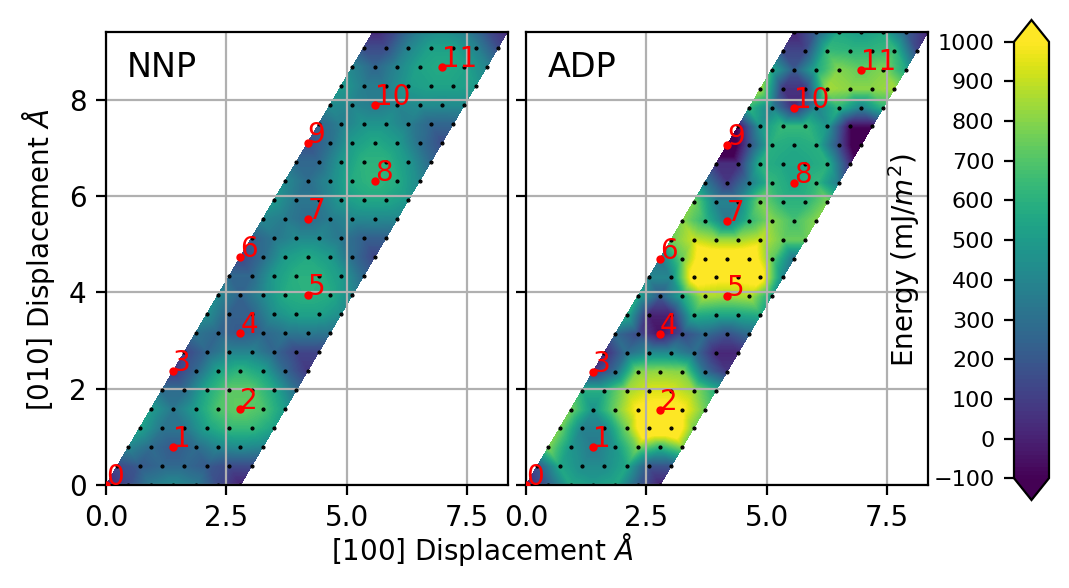
\includegraphics[scale=1.2]{figures/GSF_ThetaDP111_surf.png}
 }}%
\end{figure}


Antisites were computed for every OQMD structure in the following manner.
Firstly, the structure was allowed to be completely relaxed.
If the structure maintained the same symmetry group after full cell and atomic relaxation, we analyzed it for unique atomic sites using pymatgen.
Then the cell was duplicated, such as to generate cells with a minimum of 108 atoms to minimize defect-defect interactions.
For each of the unique sites identified, we then swapped it with the different atom, e.g., Al->Cu or Cu->Al, else we deleted the site to generate a vacancy and stored the antisite structure.
The energies of all antisite structures were calculated without relaxation.
This equation gave the antisite formation energies $H^{anti}f$:
\begin{equation}
H^{anti}f = E_{anti} - E_{pristine} - \sum\Delta n_i E^{bulk}_i
\end{equation}
Where $E_{anti}$, $E_{pristine}$ are the total energies of the antisite, and pristine structure, $n_i$ is the 
number and sign of the swapped atoms, and $E^{bulk}_i$ their groundstate energy of the bulk compound, i.e., FCC for 
both Cu and Al.

Figure \ref{fig:antisite_plot} shows the antisite results.
NNP attains excellent accuracy despite the lack of training data.
Error bars rarely exceed 5meV and are almost always centered around the correct DFT value.
ADP also performs reasonably but has substantially more errors, with many samples deviating more than 10meV/atom from DFT. 


\begin{figure}[H]%
\centering%
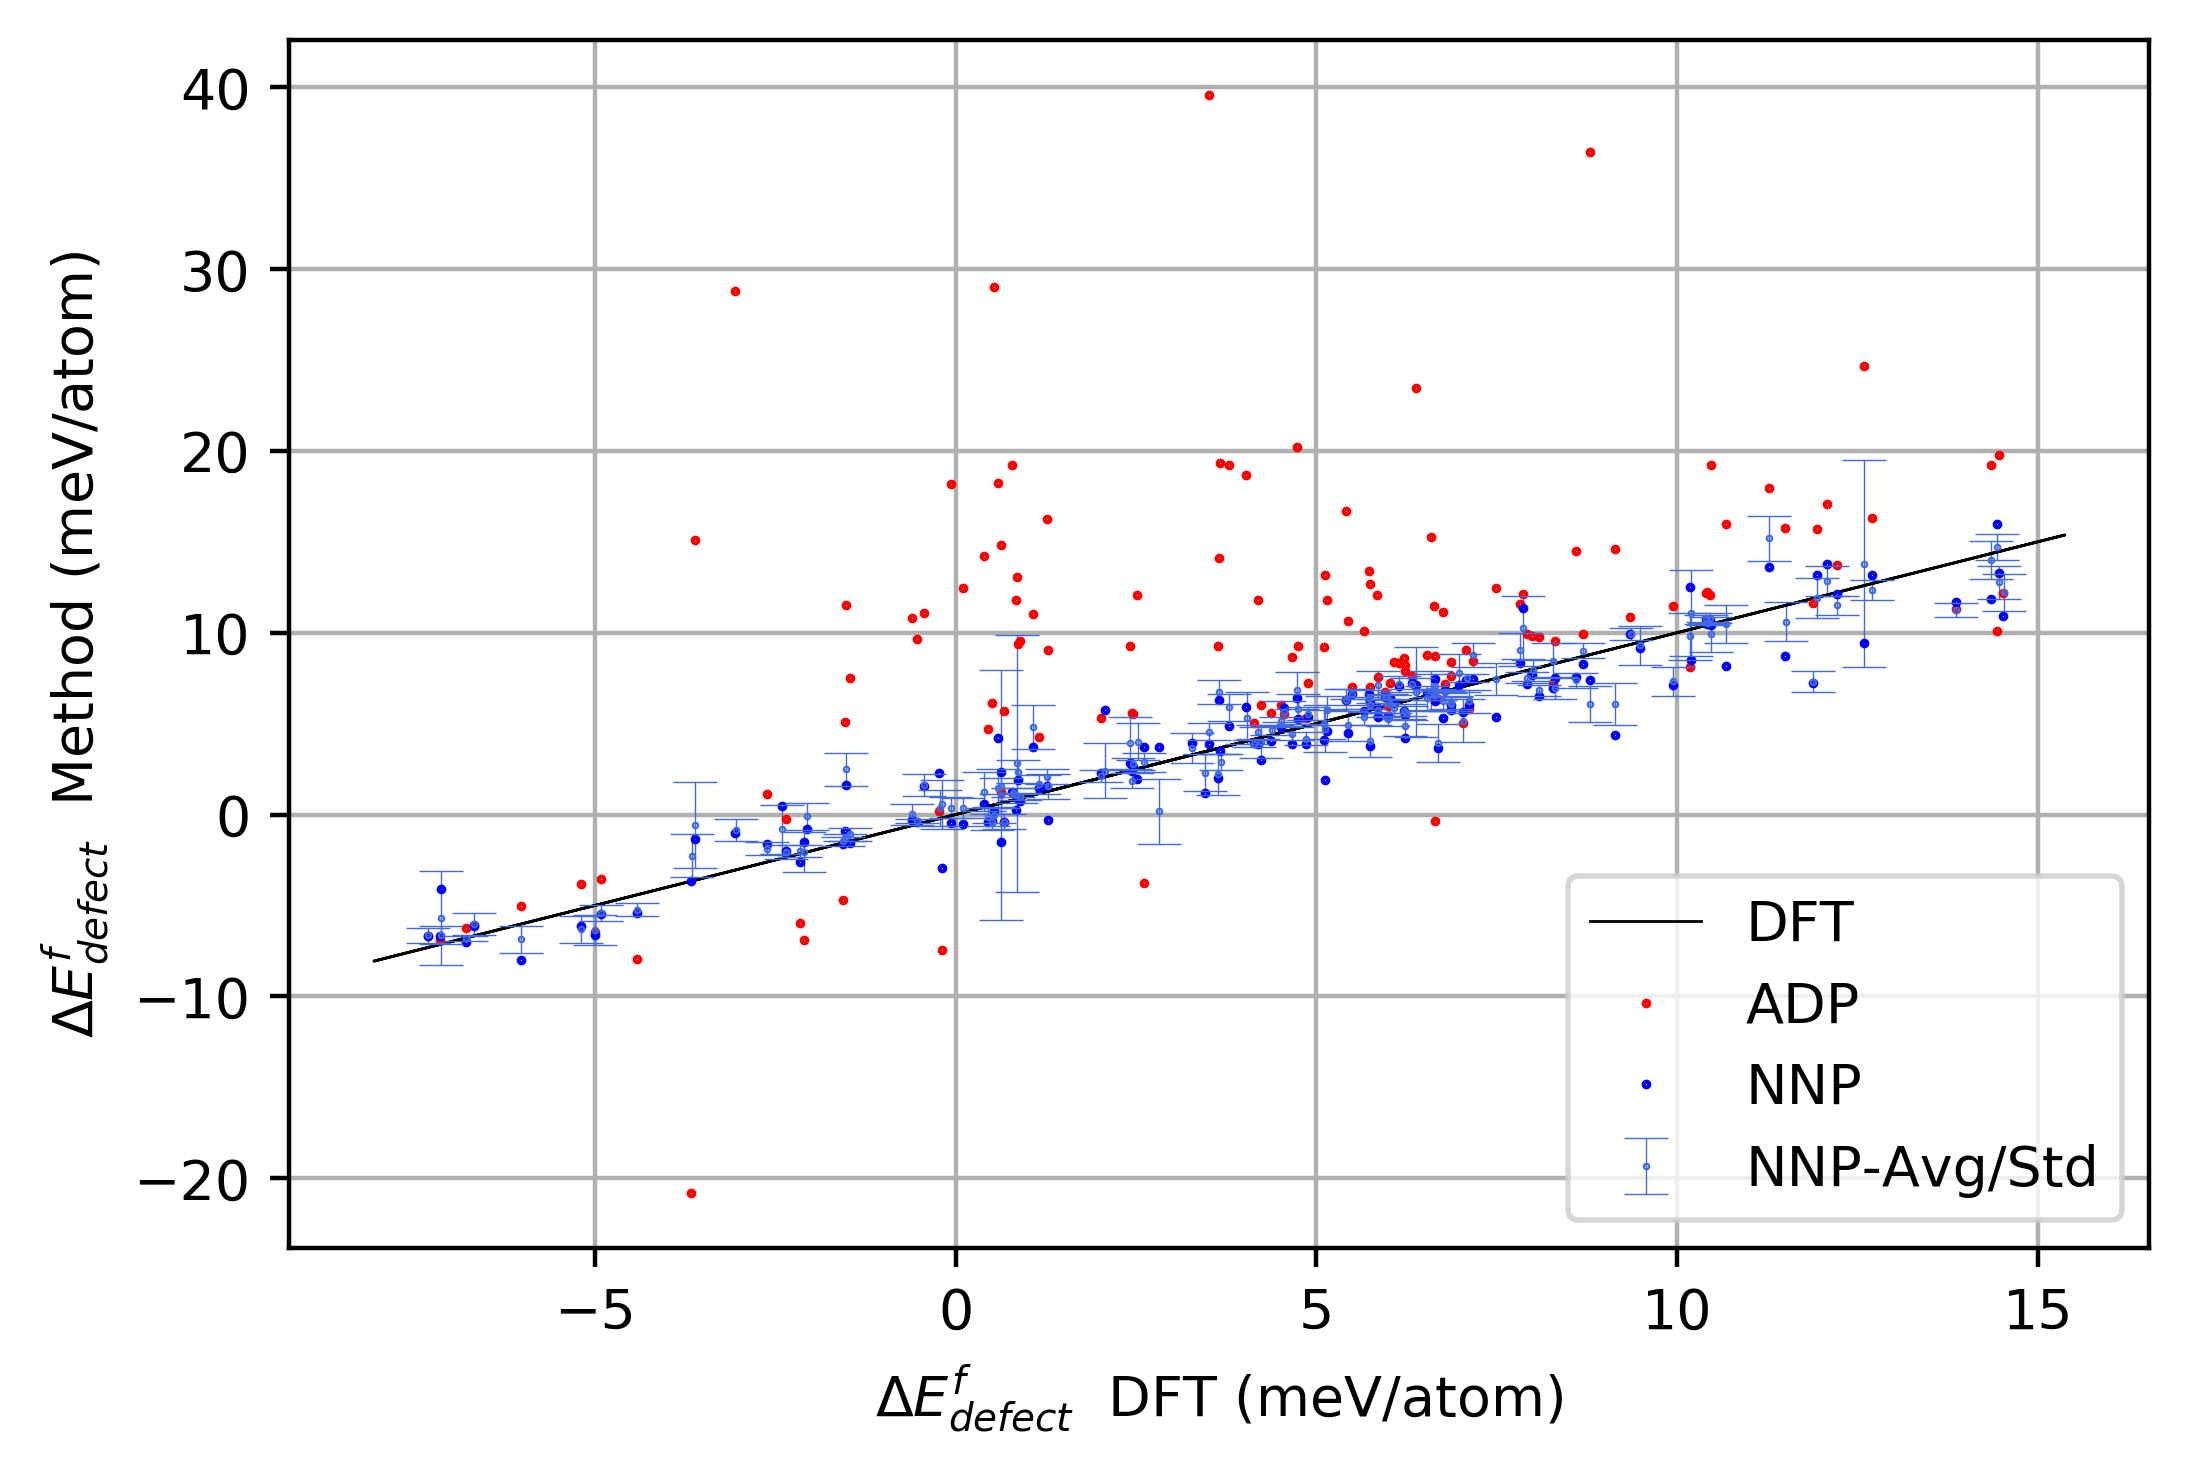
\includegraphics[width=1.2\textwidth,center]{./figures/antisite_plot.png}%
\caption{DFT antisite formation energy vs ADP/NNP antisite formation energy.
These structures were not included in the training set.}%
\label{fig:antisite_plot}
\end{figure}

\newpage
\bibliographystyle{unsrt}  
\bibliography{references}  %%% Remove comment to use the external .bib file (using bibtex).
%%% and comment out the ``thebibliography'' section.

\newpage
\appendix
\section{Supplementary}
\begin{figure}[H]%
\centering%
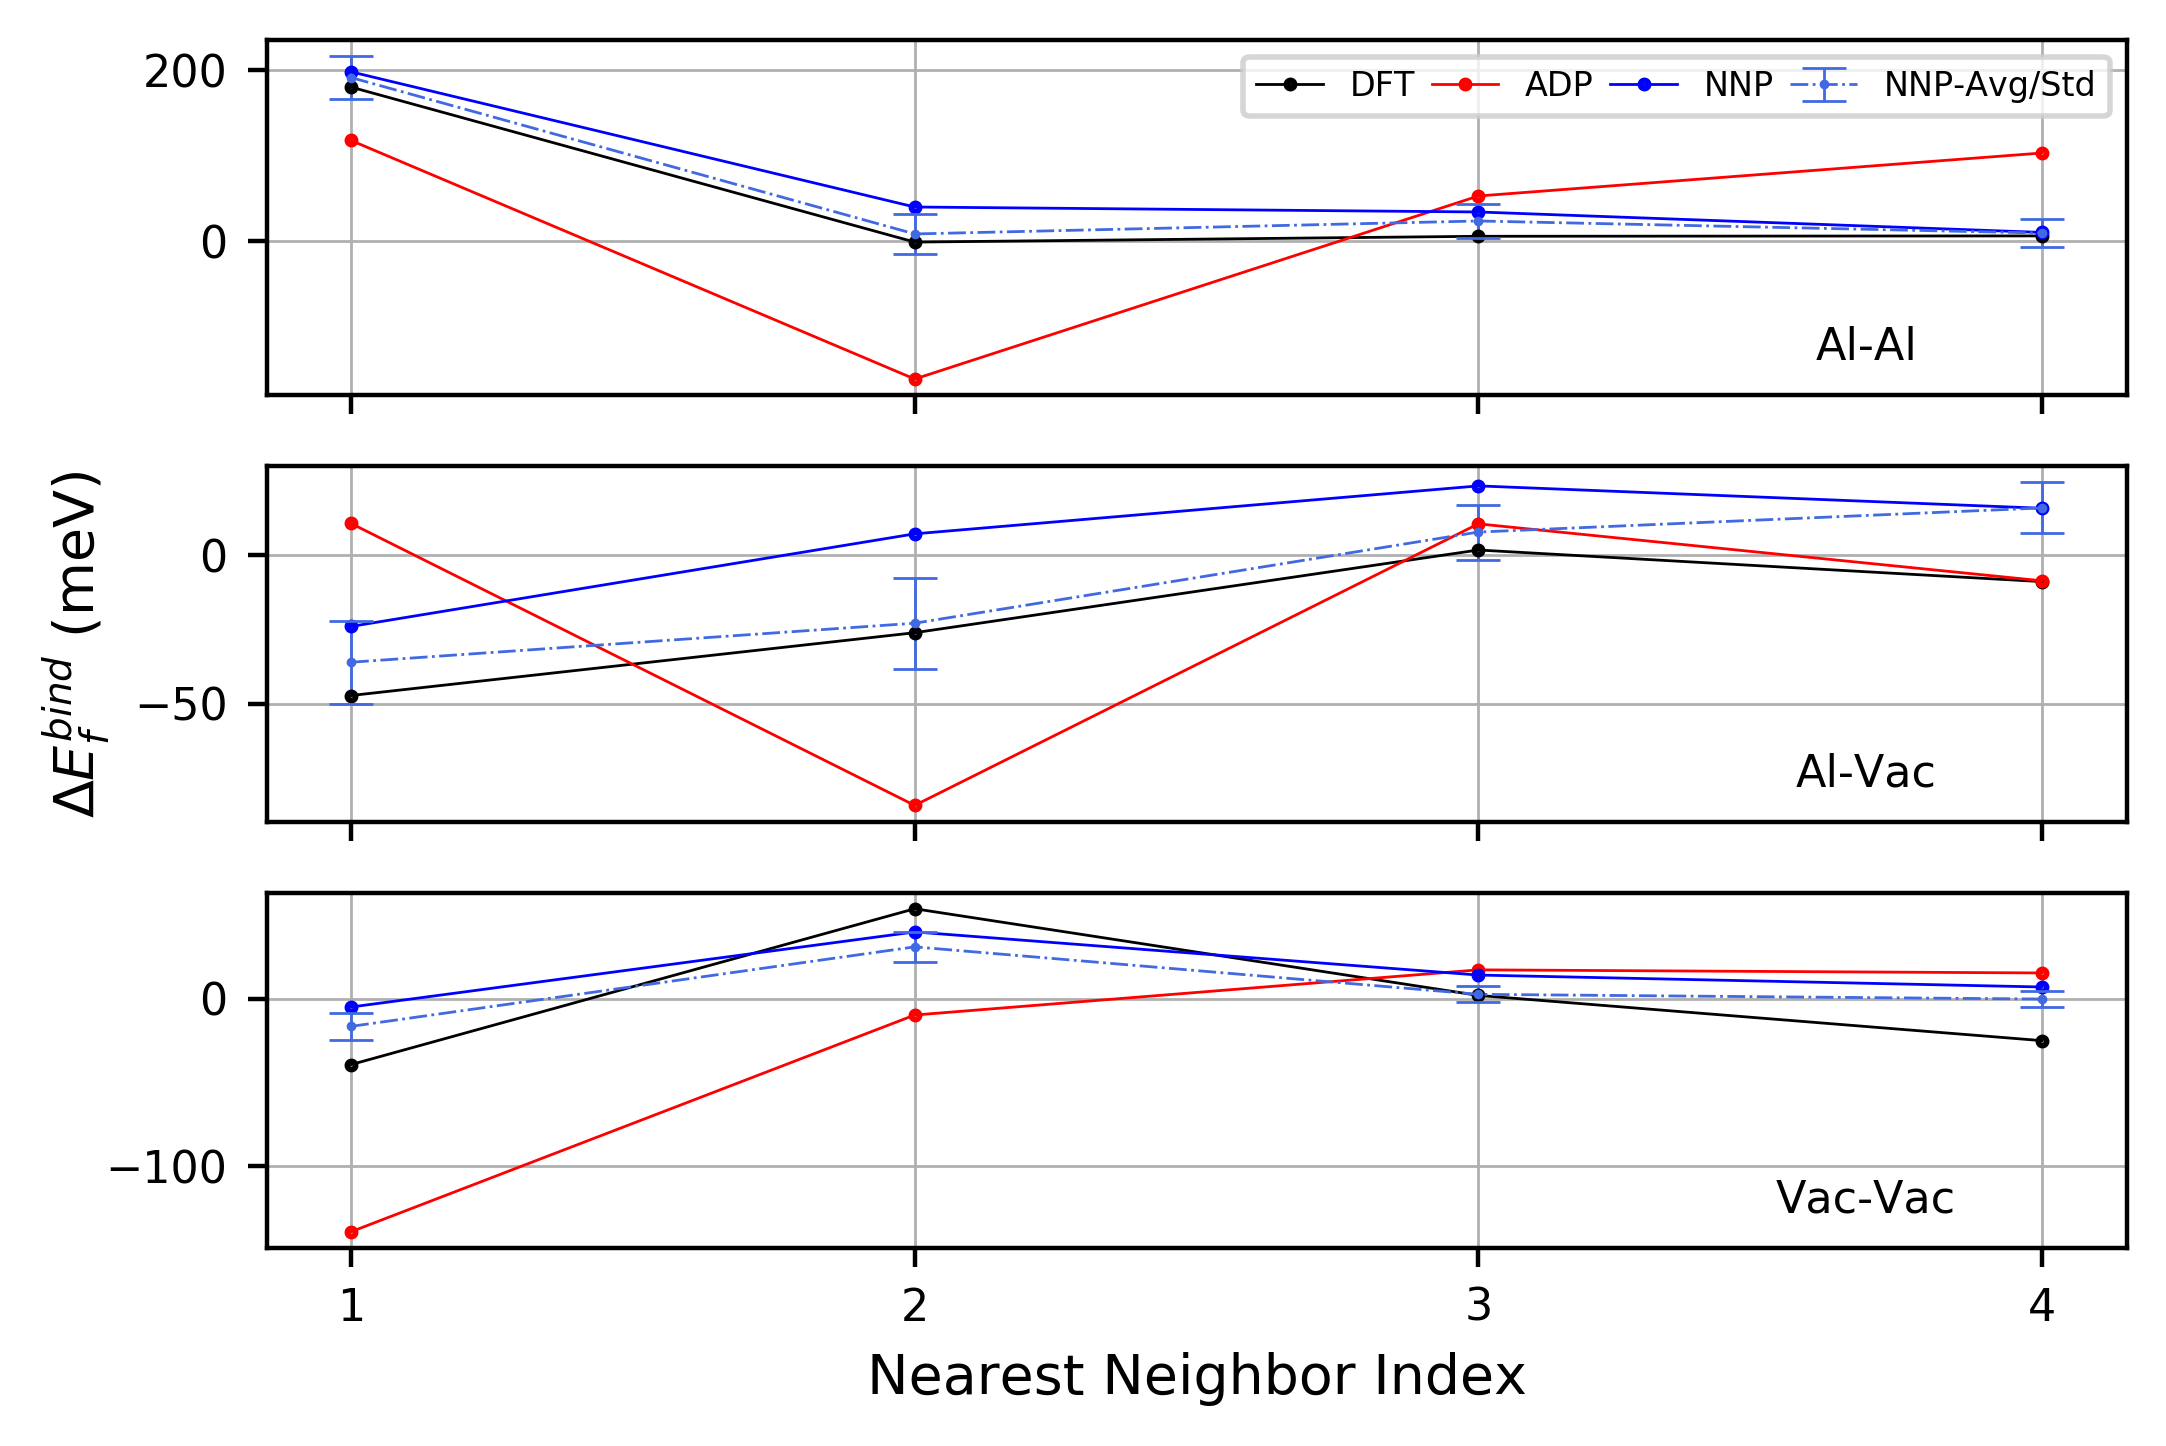
\includegraphics[width=1.2\textwidth,center]{./figures/solsol_in_cu.png}%
\caption{Neighbor index vs binding energy $E_{bind}$ for Al-Al, Al-Vac and Vac-Vac in Cu matrix.}%
\label{fig:solsol_in_cu}
\end{figure}


\begin{figure}[H]%
\centering%
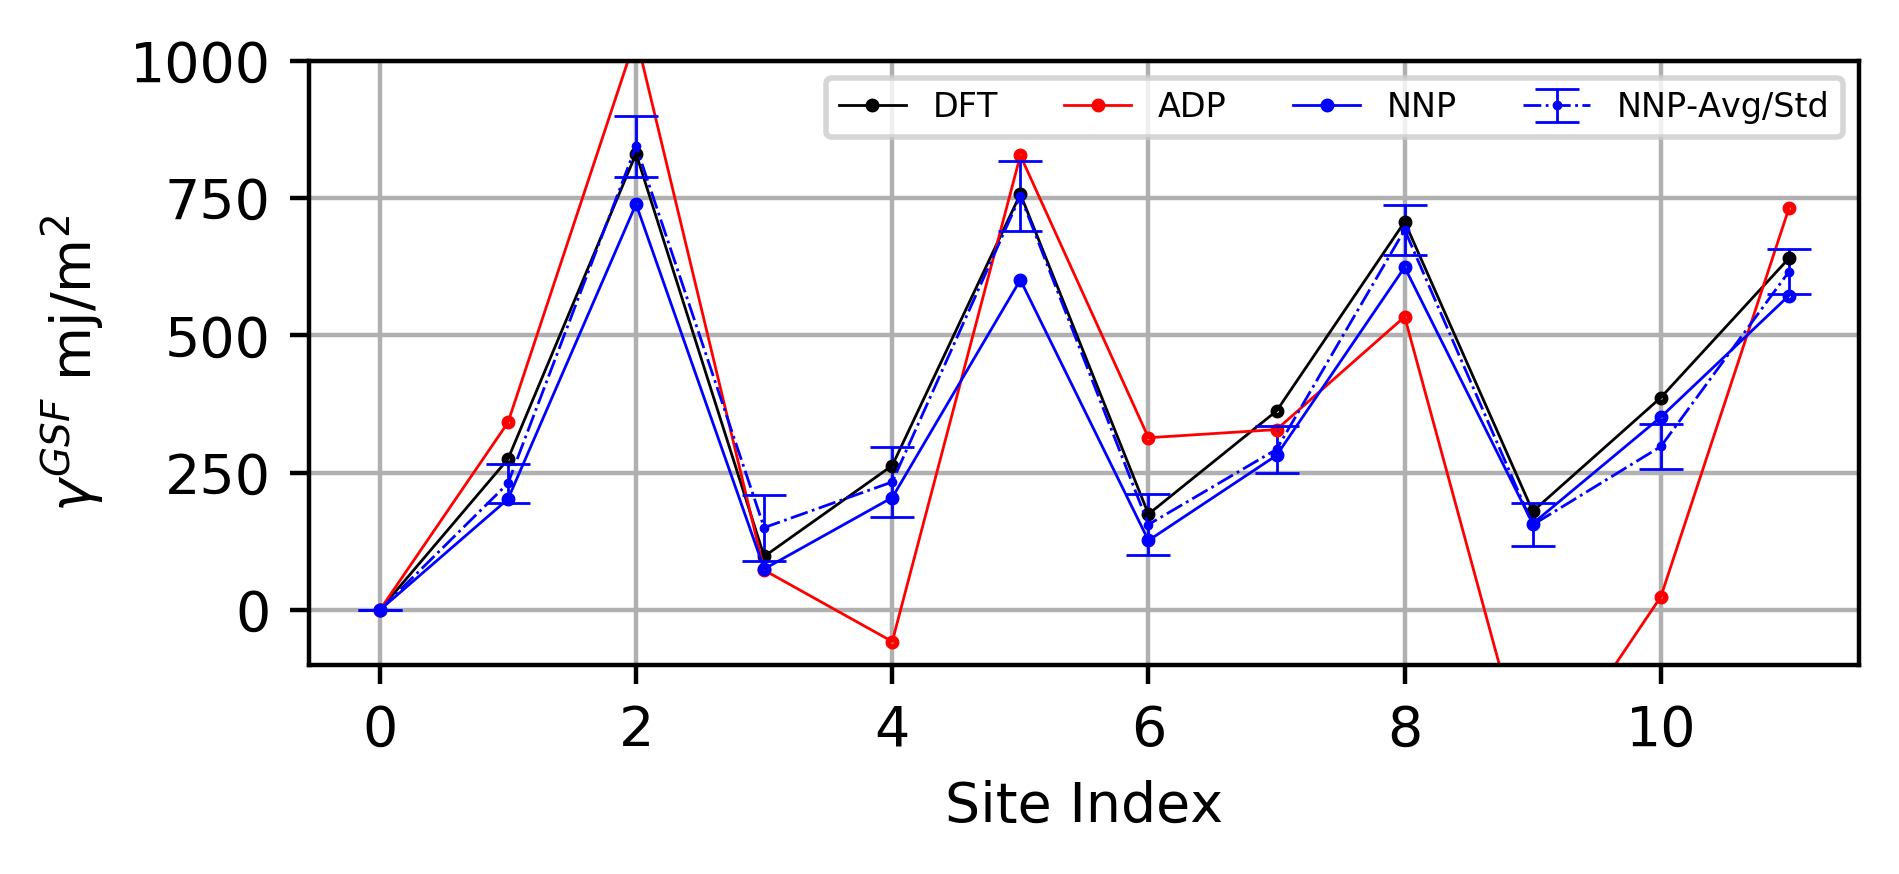
\includegraphics[width=540px]{./figures/NOTINOQMD_00002-GSF_111.png}%
\caption{GSF energy for key sites on the 111 surface of  $\theta''$.These sites are not included in the  training set for NNP}%
\end{figure}

\begin{figure}[H]%
\centering%
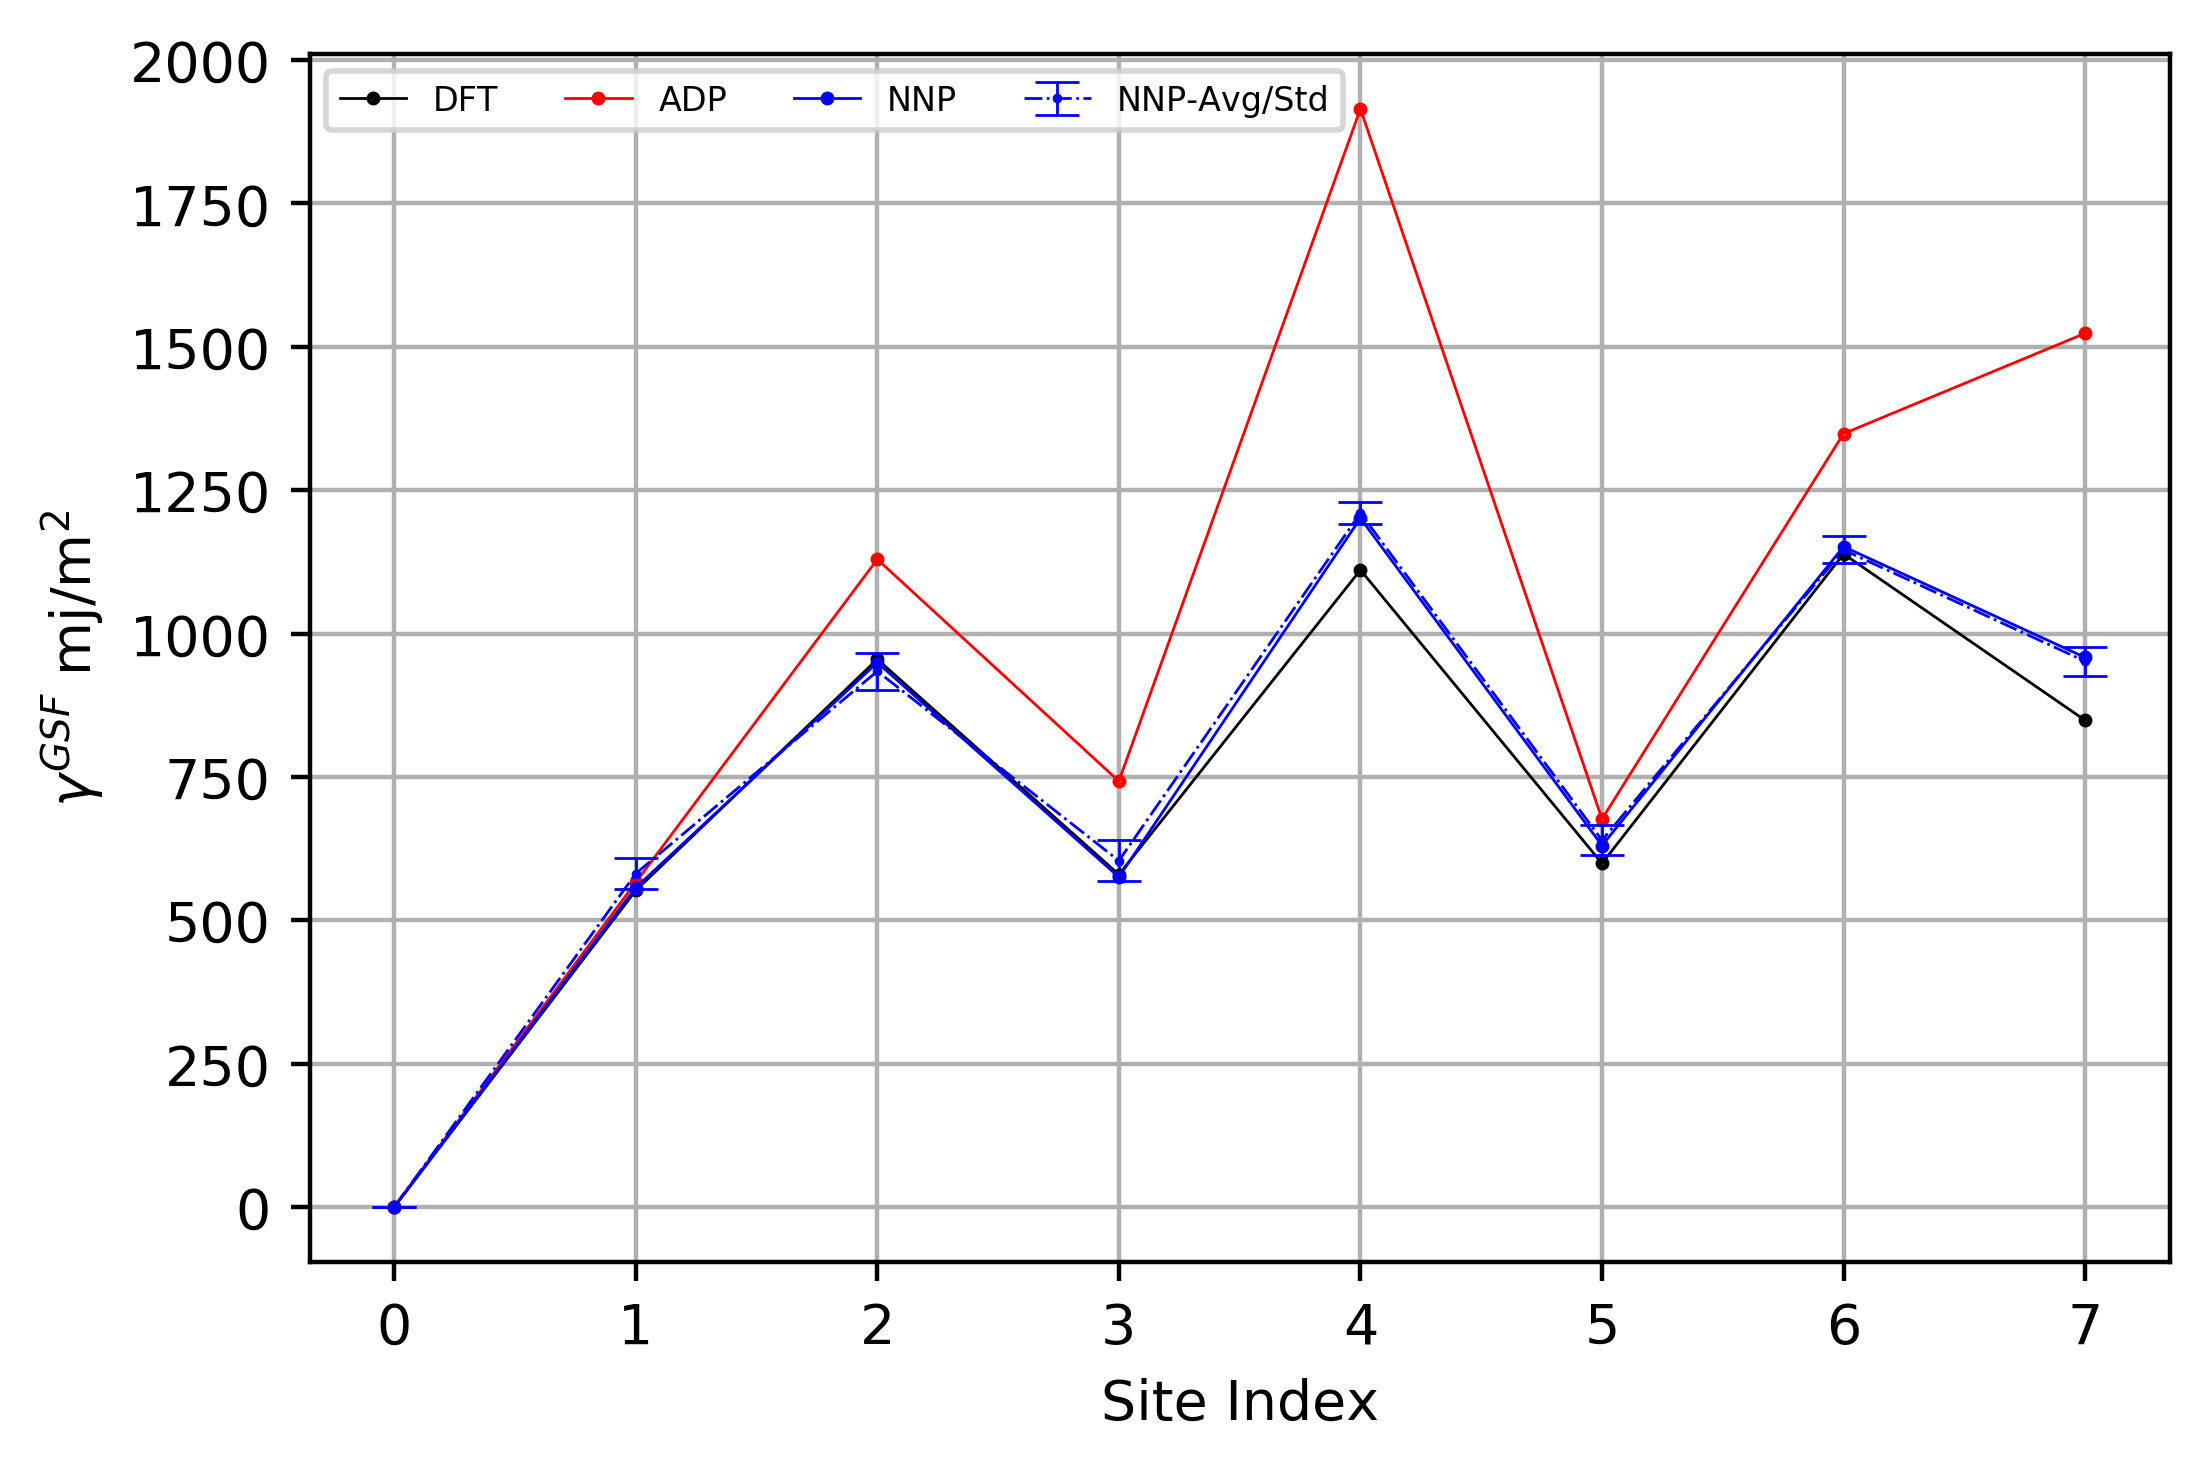
\includegraphics[width=540px]{./figures/NOTINOQMD_00001-GSF_0m11.png}%
\caption{GSF energy for key sites on the 0-11 surface of  $\theta$. These sites are included in the training set for NNP}%
\end{figure}


\begin{tabular}{l|lll|lll}%
\hline%
Structure&\multicolumn{3}{c}{FCC Al}&\multicolumn{3}{c}{FCC Cu}\\%
Method&DFT&NNP&ADP&DFT&NNP&ADP\\%
\hline%
a ($\AA$)&4.04&4.047&4.05&3.625&3.627&3.615\\%
vol/atom ($\AA^3$)&16.48&16.58&16.61&11.9&11.93&11.81\\%
G (GPa)&30.7&33.0&29.6&59.4&62.6&55.3\\%
K (GPa)&78.2&77.2&78.5&143.9&146.3&138.9\\%
$C_{11}$ (GPa)&112.5&110.6&113.5&180.3&182.4&170.4\\%
$C_{21}$ (GPa)&61.0&60.5&61.1&125.7&128.2&123.2\\%
$C_{44}$ (GPa)&34.0&38.2&31.9&80.8&86.3&76.5\\%
\hline%
\end{tabular}%
\newline%
\newline%
\newline%
\newline%

\begin{tabular}{l|ccc|ccc|ccc}%
\hline%
Structure&\multicolumn{3}{c}{Al$_2$Cu  $\theta$}&\multicolumn{3}{c}{Al$_2$Cu $\theta'$}&\multicolumn{3}{c}{Al$_3$Cu $\theta''$}\\%
Method&DFT&NNP&ADP&DFT&NNP&ADP&DFT&NNP&ADP\\%
\hline%
a ($\AA$)&4.869&4.917&4.862&4.087&4.095&3.994&2.804&2.792&2.784\\%
b ($\AA$)&4.926&4.929&4.862&4.087&4.095&3.994&2.804&2.792&2.784\\%
c ($\AA$)&4.926&4.929&4.862&4.087&4.095&3.994&7.65&7.65&7.586\\%
$\alpha$&75.9&75.6&75.2&60.0&60.0&60.0&90.0&90.0&90.0\\%
$\beta$&60.4&60.1&75.2&60.0&60.0&60.0&90.0&90.0&90.0\\%
$\gamma$&60.4&60.1&60.6&60.0&60.0&60.0&90.0&90.0&90.0\\%
vol/atom ($\AA^3$)&14.88&14.95&14.41&16.09&16.18&15.02&15.04&14.9&14.69\\%
$\Delta$$H^{comp}$ (meV/atom)&{-}161.6&{-}162.9&{-}189.8&{-}184.0&{-}184.0&{-}202.6&{-}94.2&{-}94.8&{-}128.8\\%
G (GPa)&42.3&39.3&57.5&56.6&56.5&44.1&48.8&40.6&32.6\\%
K (GPa)&100.8&115.7&154.5&97.0&96.8&138.6&94.3&89.5&84.9\\%
$C_{11}$ (GPa)&170.4&167.8&199.5&158.7&160.4&192.4&160.5&148.6&115.4\\%
$C_{22}$ (GPa)&170.4&167.8&199.5&158.7&160.4&192.4&160.5&148.6&115.4\\%
$C_{33}$ (GPa)&174.8&180.4&278.2&158.7&160.4&192.4&181.8&154.1&142.0\\%
$C_{44}$ (GPa)&28.8&37.0&80.0&63.5&62.3&46.5&45.8&32.4&38.2\\%
$C_{55}$ (GPa)&28.8&37.0&80.0&63.5&62.3&46.5&45.8&32.4&38.2\\%
$C_{66}$ (GPa)&47.5&38.1&21.0&63.5&62.3&46.5&42.2&46.6&27.4\\%
$C_{21}$ (GPa)&73.7&104.2&99.3&66.2&64.9&111.6&70.9&61.6&48.0\\%
$C_{31}$ (GPa)&61.1&79.2&128.7&66.2&64.9&111.6&51.1&57.6&73.8\\%
$C_{32}$ (GPa)&61.1&79.2&128.7&66.2&64.9&111.6&51.1&57.6&73.8\\%
\hline%
\end{tabular}%



\end{document}
